%+----------------------------------------------------------------------------+
%| SLIDES: Multisymplectic geometry, moment maps and reduction.
%| Contents:	- 60 minutes (extimated duration 4 minutes per slide, 15 slides )
%|
%| Author: Antonio miti
%| Event: oberseminar
%| Place: Bonn
%| Date: 7/4/22
%+----------------------------------------------------------------------------+


%- HandOut Flag -----------------------------------------------------------------------------------------
	\newif\ifHandout
	\Handouttrue  %uncomment for the printable version
	%Handling of flags it is not preserved when passing to standalone-subfiles!


%- D0cum3nt ----------------------------------------------------------------------------------------------
\ifHandout
	\documentclass[handout,10pt]{beamer}   
	\setbeameroption{show notes} %print notes   
\else
	\documentclass[10pt]{beamer}
\fi




%- Packages ----------------------------------------------------------------------------------------------
\usepackage{custom-style}
\usepackage{math}


%--Beamer Style-----------------------------------------------------------------------------------------------
\usetheme{toninus}


\usetikzlibrary{backgrounds}
  \tikzset{
    invisible/.style={opacity=0},
    visible on/.style={alt=#1{}{invisible}},
    alt/.code args={<#1>#2#3}{%
      \alt<#1>{\pgfkeysalso{#2}}{\pgfkeysalso{#3}} % \pgfkeysalso doesn't change the path
    },
  }


%- T1tle P4g3 -------------------------------------------------------------------------------------------
\title{ Symmetries and Reduction \\ of Multisymplectic Manifolds } 
\subtitle{\href{https://www.mpim-bonn.mpg.de/node/158}{MPI-Oberseminar}}
\author[AMM]{\href{https://dmf.unicatt.it/miti/}{Antonio Michele Miti}}
%\institute[UCSC and KU Leuven]{
%  \begin{tabular}[h]{ccc}
%      Università Cattolica del Sacro Cuore & $\qquad$ & KU Leuven \\
%      Brescia, Italy & & Leuven, Belgium \\
%      \href{https://dipartimenti.unicatt.it/dmf-home?rdeLocaleAttr=it}{
\includegraphics[width=3.5cm]{Logos/UnicattBS-logo}} & & 
%      \href{https://wis.kuleuven.be/english}{
\includegraphics[width=4cm]{Logos/KULeuven_logo}}
%  \end{tabular}      
%}
\institute[Mpim]{
	MPIM, Bonn, Germany 
	\\
	\vspace{.5em}
	\href{https://www.mpim-bonn.mpg.de/}{
\includegraphics[width=6cm]{./Logos/Mpim_logo}}
}
\date[Template_21] % (optional, should be abbreviation of conference name)
{	
	{\vskip 1ex}
	Bonn, April 7, 2022
}












%---------------------------------------------------------------------------------------------------------------------------------------------------
%- D0cum3nt ----------------------------------------------------------------------------------------------------------------------------------
\begin{document}
%-------------------------------------------------------------------------------------------------------------------------------------------------
\begin{frame}  % Alternative: \maketitle outside of frame
	\titlepage
	\ifHandout
		\tikz[overlay,remember picture]
		{
	    	%	\node at ($(current page.west)+(1.5,0)$) [rotate=90] {\Huge\textcolor{gray}{\today}};
	    	\node[        
	    		draw,
	    		shape border rotate=90,
			isosceles triangle,
			isosceles triangle apex angle=90,
			fill=yellow]
	        		at ($(current page.north east)-(1,1)$) [rotate=-45] {\textcolor{red}{Handout version}};
		}
	\fi
	\end{frame}
	\addtocounter{framenumber}{-1}
\note{
	%\textbf{\underline{OUTLINE}}:
	%\tableofcontents
	\textbf{Abstract:}
	\\
%
Multisymplectic manifolds are a straightforward generalization of symplectic manifolds where closed non-degenerate k-forms are considered in place of 2-forms.
A natural theme that arises when dealing with (multi)symplectic structures is investigating the relationship between symmetries (group action preserving the fixed differential form) and reduction.

In this context, a reduction scheme can be taught as a procedure to construct a second space of reduced dimension out of a given (multi)-symplectic manifold with symmetries. The so obtained reduced space enjoys the convenient property of embodying the relevant geometric structure of the starting unreduced object.

A well-known result in symplectic geometry, known as Marsden–Weinstein–Meyer theorem, states that the relevant geometric structure of a symplectic manifold can be studied on the orbits contained in a regular level set of a so-called "momentum map".
Sniaticki and Weinstein have further extended this result to encompass singular momentum maps.

The scope of this talk is to review some relevant algebraic structures related to multisymplectic manifolds, namely the higher version of the observables algebra and moment maps, and discuss how the regular and singular reduction schemes extend to the multisymplectic framework.

This talk is based on ongoing joint work with Casey Blacker and Leonid Ryvkin.

}
%---------------------------------------------------------------------------------------------------------------------------------------------------





%-------------------------------------------------------------------------------------------------------------------------------------------------
\section{Introduction}
%-------------------------------------------------------------------------------------------------------------------------------------------------
	%- HandOut Flag -----------------------------------------------------------------------------------------
\makeatletter
\@ifundefined{ifHandout}{%
  \expandafter\newif\csname ifHandout\endcsname
}{}
\makeatother

%- D0cum3nt ----------------------------------------------------------------------------------------------
\documentclass[beamer,10pt]{standalone}   
%\documentclass[beamer,10pt,handout]{standalone}  \Handouttrue  

\ifHandout
	\setbeameroption{show notes} %print notes   
\fi

	
%- Packages ----------------------------------------------------------------------------------------------
\usepackage{custom-style}
\usetikzlibrary{positioning}
\usepackage{multicol}


%--Beamer Style-----------------------------------------------------------------------------------------------
\usetheme{toninus}
\usepackage{animate}
\usetikzlibrary{positioning, arrows}
\usetikzlibrary{shapes}


% ==========================================================================================
\begin{document}
% ==========================================================================================

%-------------------------------------------------------------------------------------------------------------------------------------------------
\begin{frame}[fragile]{Keywords}
\tikzstyle{every picture}+=[remember picture]
	\begin{columns}
    	\begin{column}{.45\textwidth}
    		\onslide<3->{
			\tikz[baseline]{
		            \node[draw=orange!40,anchor=base,text width=5cm] (s1)
		            {Group of transformations preserving the prescribed geometric structures.};
			}
		}
	\end{column}
    	\begin{column}{.45\textwidth}
    		\onslide<4->{
			 \tikz[baseline]{
		            \node[draw=blue!40,anchor=base, text width=5cm] (s2)
		            {Procedure providing another manifold of reduced dimension encoding the relevant geometrical information.};
			}
		}
	\end{column}
	\end{columns}

	\vfill

	\begin{center}
		\large
		 \tikz[baseline]{
		            \node[fill=orange!20,anchor=base] (t1)
		            {Symmetries};
			}
		 and
		 \tikz[baseline]{
		            \node[fill=blue!20,anchor=base] (t2)
		            {Reduction};
		        } 
		\\
		of 
		 \tikz[baseline]{
	            \node[fill=green!20,anchor=base] (t3)
	            {Multi};
		}
		\kern-3pt - \kern-3pt
		 \tikz[baseline]{
	            \node[fill=red!20,anchor=base] (t4)
	            {Symplectic};
		}		
        manifolds
	\end{center}

	\vfill

	\begin{columns}
    	\begin{column}{.45\textwidth}
    		\onslide<2->{
	 		 \tikz[baseline]{
	            \node[draw=green!40,anchor=base,text width=5cm] (s3)
	            {A certain higher version \\(involving differential forms in degree $\geq 2$)};
	         }
		}		   	
		\end{column}
    	\begin{column}{.45\textwidth}
		\tikz[baseline]{
	            \node[draw=red!40,anchor=base,text width=5cm] (s4)
	            {Geometric structure providing a prescription on how to measure the area of 2-dimensional surface elements embedded in the manifold.};
		}	
		\end{column}
	\end{columns}

	\begin{tikzpicture}[overlay]
        \path[->,draw=orange!40]<3-> (s1) edge [bend right] (t1);
        \path[->,draw=blue!40]<4-> (s2) edge [bend left] (t2);
        \path[->,draw=green!40]<2-> (s3) edge [bend left] (t3);
        \path[->,draw=red!40] (s4) edge [bend right] (t4);
	\end{tikzpicture}

\end{frame}
\note[itemize]{
	\item Provide a vague idea of the words that make up the title.
}
%-------------------------------------------------------------------------------------------------------------------------------------------------


%-------------------------------------------------------------------------------------------------------------------------------------------------
\begin{frame}{Symplectic geometry (mechanics flavour)}
\begin{columns}[T]
	\begin{column}{.50\linewidth}
		\centering
		\textit{ "geometric approach" to mechanics \dots}
		%
		\begin{columns}
			\begin{column}{.60\linewidth}
				\begin{center}
					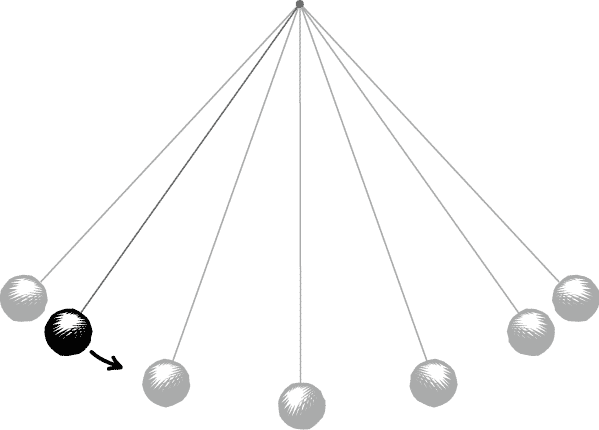
\includegraphics[width=0.6\linewidth]{Pictures/pendulum13}			
				\end{center}
			\end{column}	
			\begin{column}{.40\linewidth}
				\begin{center}
					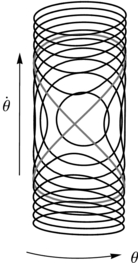
\includegraphics[width=0.45\linewidth]{Pictures/pendulum-phase-space}			
				\end{center}
			\end{column}	
		\end{columns}
		%
		\begin{defblock}[Symplectic Manifold]
			\vspace{-1em}
			\includestandalone[width=1\textwidth]{Pictures/Figure_sym}	
		\end{defblock}
		%
		\pause
		\begin{exblock}[$M = T^\ast Q$ is symplectic]
			with $\omega = d \theta $ given by
			$$ \left.\theta\right\vert_{(q,p)} (v) = p (\pi_\ast v) ~.$$
		\end{exblock}
		%
		\pause
		\vspace{1em}
		\centering
		\textit{ based on the notion of \\"states".}		
	\end{column}
	\onslide<1->{\vrule{}}
	\pause
	\begin{column}{.50\linewidth}
		\centering
		\textit{ "algebraic approach" to mechanics \dots}
		\vspace{.5em}	
		\begin{defblock}[Classical Observables]
			Unital, associative, commutative algebra $C^\infty(M)$.
		\end{defblock}
		%
		\vspace{.5em}
		\pause
		\begin{defblock}[Hamiltonian vector fields]
			$v_f \in \mathfrak{X}(M)$ such that:
			$$\iota_{v_f} \omega = -df \quad \text{(exact)}$$ %$\in B^1(M)$
			\small$v_f$ = \emph{Ham.v.f. pertaining to $f\in C^\infty(M)$}.
		\end{defblock}
		%
		\begin{defblock}[Poisson Algebra of Observables]
			$C^\infty(M)$ is a Poisson algebra with
			$$\{f,g\} = \iota_{v_g} \iota_{v_f} \omega = \omega(v_f,v_g) ~.$$
		\end{defblock}
		%
		\pause
		\vspace{.8em}
		\centering
		\textit{ based on the notion of \\"meaurable quantities".}						
	\end{column}
\end{columns}
\end{frame}
\note[itemize]{
	\footnotesize

	\item We work in the framework of multisymplectic geometry which is one of the possible generalizations of the well-established field of symplectic geometry.
	
	\item To recall what symplectic geometry is let me assume a particular point of view: mechanics.
	\\
	Idea:"
	Symplectic geometry is a branch of differential geometry studying symplectic manifolds; it originated as a formalization of the mathematical apparatus of classical mechanics and geometric optics."{\href{https://ncatlab.org/nlab/show/symplectic+geometry}{nlab}}
	
	Namely, a sym. mfd. is the geometric structure encoding the phase space of conservative, ordinary, classical, mechanical systems.
	
	\item $\theta$ = \emph{tautological 1-form}.
		$\theta$ evaluated at $p\in T^*Q$ in the fibre of $q\in Q$ and contracted with $v$ coincides with the form $p$ evaluated at $q$ and contracted with the push forward of $v$.
	
	\item We identify a special class of vector fields.
		Out of them one can define a Lie bracket.
	
	\item Poisson is a Lie algebra with the extra property of compatibility with the associative product (Leibniz rule)
	
	\item take away message: geometric (based on "states") vs algebraic (based on "measurable quantities").7
}
%-------------------------------------------------------------------------------------------------------------------------------------------------



%-------------------------------------------------------------------------------------------------------------------------------------------------
\begin{frame}{From symplectic to {multi}symplectic} 
	%
	\begin{center}
		$-$ \emph{multisymplectic means \textbf{going higher} in the degree of $\omega$} $-$
	\end{center}
	\pause
	\begin{defblock}[$n$-plectic manifold ~\emph{(Cantrijn, Ibort, De Le\'on)} \cite{Cantrun2017}]
		\includestandalone[width=0.95\textwidth]{Pictures/Figure_multisym}	
	\end{defblock}
	%
	\pause
		\begin{table}
			\begin{tabular}{c c c}
				symplectic forms \small($n=1$) & $\leftrightsquigarrow$ & volume forms \small($n= \text{dim}(M)-1$)
			\end{tabular}
		\end{table}

	\vfill
	\pause
	\begin{block}{Historical motivation}
		Mechanics: geometrical foundations of \textit{(first-order)} field theories.
	\end{block}
	\begin{table}
		\only<4>{
		\begin{tabular}{|p{0.2\textwidth}|p{0.3\textwidth}|p{0.35\textwidth}|} 
            \hline
            \parbox[][20pt][c]{0.2\textwidth}{mechanics} & \multicolumn{2}{c|}{geometry} \\
            \hline
            \parbox[][20pt][c]{0.2\textwidth}{phase space} & symplectic manifold &  \\[.25em]
            \parbox[][20pt][c]{0.2\textwidth}{classical \\ observables} & Poisson algebra &  \\[.25em]
            \parbox[][20pt][c]{0.2\textwidth}{symmetries} &  group actions admitting comoment map &  
            \\
            \hline
  \multicolumn{1}{c}{}
            &  \multicolumn{1}{@{}c@{}}{$\underbrace{\hspace*{.3\textwidth}}_{\text{point-like particles systems}}$} 
            &  \multicolumn{1}{@{}c@{}}{}              \\
		\end{tabular}
		
		
		}
		\onslide<5->{
		\begin{tabular}{|p{0.2\textwidth}|p{0.3\textwidth}|p{0.35\textwidth}|} 
            \hline
            \parbox[][20pt][c]{0.2\textwidth}{mechanics} & \multicolumn{2}{c|}{geometry} \\
            \hline
            \parbox[][20pt][c]{0.2\textwidth}{phase space} & symplectic manifold & multisymplectic manifold \\[.25em]
            \parbox[][20pt][c]{0.2\textwidth}{classical \\ observables} & Poisson algebra & $L_\infty$-algebra \\[.25em]
            \parbox[][20pt][c]{0.2\textwidth}{symmetries} &  group actions admitting comoment map & group actions admitting (homotopy) comomentum map
            \\
            \hline
  			\multicolumn{1}{c}{}
            &  \multicolumn{1}{@{}c@{}}{$\underbrace{\hspace*{.3\textwidth}}_{\text{point-like particles systems}}$} 
            &
            \multicolumn{1}{@{}c@{}}{$\underbrace{\hspace*{.3\textwidth}}_{\text{field-theoretic systems}}$} 
               \\
		\end{tabular}
		}
	\end{table}	




\end{frame}
\note[itemize]{
	\item Historically, the interest in multisymplectic manifolds, has been motivated by the need for understanding the geometrical foundations of first-order classical field theories.
	The key point is that, just as one can associate a symplectic manifold to an ordinary classical mechanical system (e.g. a single
point-like particle constrained to some manifold), it is possible to associate a multisymplectic
manifold to any classical field system (e.g. a continuous medium like a filament or a fluid). See frame Extra-\ref{Frame:Ms-Field-Mechanics} 
	
	\item General ideas basic parallelisms with caveats
	\item caveat: points in multiphase spaces are not states
	\item the table hides the duality between geometric and algebraic approaches to the problem.
	\item	Mechanics: geometrical foundations of \textit{(first-order)} field theories.
		\begin{itemize}
		 \item[-] Kijowski, W. Tulczyjew \cite{Kijowski1979}; %(1979)
		 \item[-] Cariñena, Crampin, Ibort \cite{Carinena1991b};% (1991)
		 \item[-] Gotay, Isenberg, Marsden, Montgomery \cite{Gimmsy1};%(1998)
		 \\ $\cdots$
		\end{itemize}
}
%-------------------------------------------------------------------------------------------------------------------------------------------------






% ==========================================================================================
\end{document}
% ==========================================================================================


%-------------------------------------------------------------------------------------------------------------------------------------------------
\begin{frame}{Scope of the talk} 
	    		\tableofcontents


		\tikz[overlay,remember picture]
		{
			\node[draw,
					ellipse callout,
					red, 
					minimum height=6em,
					minimum width=14em,
					callout relative pointer={(-2.25,-.15)}
			] (base1) at ($(current page.north east)-(3,2.25)$) {};
			\node
            	 [rotate=-0,
    	        	 text width=16em,
            	 text centered, 
            	 color=black] 
            	 (text) at (base1)
            	 {
	            	 Review the basics of multisym. geometry.
            	 };

			\node[draw,
					ellipse callout,
					red, 
					minimum height=6em,
					minimum width=14em,
					callout relative pointer={(-.5,-.05)}
			] (base2) at ($(current page.east)-(3,0)$) {};
			\node
            	 [rotate=-0,
    	        	 text width=16em,
            	 text centered, 
            	 color=black] 
            	 (text) at (base2)
            	 {
	            	 Discuss the \underline{regular reduction} scheme in multisym. geometry.
            	 };

			\node[draw,
					ellipse callout,
					red, 
					minimum height=6em,
					minimum width=14em,
					callout relative pointer={(-2.25,.4)}
			] (base3) at ($(current page.east)-(3,3)$) {};
			\node
            	 [rotate=-0,
    	        	 text width=16em,
            	 text centered, 
            	 color=black] 
            	 (text) at (base3)
            	 {
	            	 Discuss the \underline{singular reduction} scheme in multisym. geometry.
            	 };
		}	

\end{frame}
\note[itemize]{
	\item
}
%-------------------------------------------------------------------------------------------------------------------------------------------------






%-------------------------------------------------------------------------------------------------------------------------------------------------
\section{Multisymplectic Geometry}
\checkpoint	
%-------------------------------------------------------------------------------------------------------------------------------------------------
	%- HandOut Flag -----------------------------------------------------------------------------------------
\makeatletter
\@ifundefined{ifHandout}{%
  \expandafter\newif\csname ifHandout\endcsname
}{}
\makeatother

%- D0cum3nt ----------------------------------------------------------------------------------------------
\documentclass[beamer,10pt]{standalone}   
%\documentclass[beamer,10pt,handout]{standalone}  \Handouttrue  

\ifHandout
	\setbeameroption{show notes} %print notes   
\fi

	
%- Packages ----------------------------------------------------------------------------------------------
\usepackage{custom-style}
\usepackage{math}
\usetikzlibrary{positioning}
\usepackage{multicol}
\usepackage{bbold}

%--Beamer Style-----------------------------------------------------------------------------------------------
\usetheme{toninus}
\usepackage{animate}
\usetikzlibrary{positioning, arrows}
\usetikzlibrary{shapes}


%============================================================================================================
\begin{document}
%============================================================================================================


%-------------------------------------------------------------------------------------------------------------------------------------------------
\subsection{Multisymplectic manifolds}
%-------------------------------------------------------------------------------------------------------------------------------------------------
\begin{frame}[fragile]{Multisymplectic manifolds} %Fragile -->workaround tikzcd
	\begin{defblock}[$n$-plectic manifold ~\emph{(Cantrijn, Ibort, De Le\'on)}]
		\includestandalone[width=0.95\textwidth]{Pictures/Figure_multisym}	
	\end{defblock}
	%
	\begin{defblock}[Non-degenerate $(n+1)$-form]
		\begin{columns}
			\begin{column}{.45\linewidth}
				\centering{
				The $\omega^\flat$ (flat) bundle map is injective.
				}
			\end{column}
			\begin{column}{.5\linewidth}
						\vspace{-.5em}
				\[
				\begin{tikzcd}[column sep= small,row sep=0ex,
				/tikz/column 1/.append style={anchor=base east}]
				    \omega^\flat \colon T M \ar[r]& \Lambda^n T^\ast M \\
  						 (x,u) \ar[r, mapsto]& (x,\iota_{u} \omega_x)						
				\end{tikzcd}	
				\]
			\end{column}
		\end{columns}
	\end{defblock}
	%
	\vfill
	%
	\begin{block}{Examples:}
		\vspace{-.5em}
		\setbeamercovered{transparent}
		\begin{itemize}[<+->]
			\item[$\bullet$] $n=1$ \qquad\qquad\qquad $\Rightarrow$\quad $\omega$ is a symplectic form
			\item[$\bullet$]  $n=(dim(M)-1)$ \quad$\Rightarrow$\quad $\omega$ is a volume form
			%Any oriented $(n+1)$-dimensional manifold is $n$-plectic w.r.t. the volume form.
			%\item[$\bullet$] Let $G$ a semisimple Lie group and $\langle\cdot,\cdot \rangle$  its killing form. Then $\langle [\cdot,\cdot],\cdot \rangle$ extends to a biinvariant multisymplectic form $\omega$.
			\item[$\bullet$] Let $Q$ a smooth manifold, the multicotangent bundle $\Lambda^n T^\ast Q$ is naturally $n$-plectic.%
			\quad
			\textit{(cfr, \href{https://arxiv.org/abs/physics/9801019}{GIMMSY} construction for classical field theories)}
		\end{itemize}
	\end{block}			 
	
%
\end{frame}
\note[itemize]{
	\item Multisymplectic ($n$-plectic) geometry is a generalization of symplectic geometry where a closed, non degenerate $n+1$-form $(n\geq 1)$  takes the place of the symplectic 2-form
	
	\item multisymplectic means \emph{going higher} in the degree of $\omega$
	
	\item non degeneracy means $\iota_v\omega = 0 \Leftrightarrow v=0$.
	
	\item examples: 
	\\1-plectic $=$ symplectic, 
	\\any oriented $(n+1)$-dimensional manifold is $n$-plectic w.r.t. the volume form
	\\the multicotangent bundle $\Lambda^n T^\ast Q$ is naturally $n$-plectic (see frame extra-\ref{Frame:Ms-Field-Mechanics})
	
	\item Observe also that, by degree reason, when $n$ is equal to $1$ or $dim(M)+1$ an injective flat map $\flat$ is also bijective.
	
	\item It is important to stress that mechanical systems are not the only source instances of this class of of structures. 
				e.g. any semisimple Lie groups has associated a 2-plectic structure and any oriented $n+1$ dimensional manifold is naturally $n$-plectic.
				

}
%---------------------------------------------------------------------------------------------------------------------------------------------------



%------------------------------------------------------------------------------------------------
\begin{frame}[t]{Special classes of smooth objects}\label{Frame:Classes-Multisymplectic-Objects}
	\vspace{-1.5em}
  	\begin{columns}
		\begin{column}[t]{.42\linewidth}		
			\begin{defblock}[Hamiltonian v.f.]
				$\mathfrak{X}_{ham} =  \left\lbrace X \in  \mathfrak{X} \right\vert \left. \iota_x \omega \textrm{ exact}  \right\rbrace$ 			
			\end{defblock}
			\begin{defblock}[Multisymplectic v.f.]
				$\mathfrak{X}_{ms} =  \left\lbrace X \in  \mathfrak{X} \right\vert \left. \mathcal{L}_X \omega = 0  \right\rbrace$ 	
			\end{defblock}
		\end{column}
		\begin{column}[t]{.58\linewidth}		
			\begin{defblock}[Hamiltonian $(n$-$1)-$forms]
				\begin{displaymath}
					\Omega^{n-1}_{ham} 	:=
					\biggr\{ H \in  \Omega^{n-1} \; \left\vert \; 
					\stackanchor{$\exists X \in \mathfrak{X}_{ham}$}{: $d H = -\iota_X \omega$} \right\} 
			\end{displaymath}
			\end{defblock}		
		\end{column}
  	\end{columns}
  	%
  	\vfill
  	%
  	\onslide<2->{
  	\begin{columns}
		\begin{column}[t]{.5\linewidth}	
			\centering\emph{Global symmetries}
			\begin{defblock}[Multisym. (Lie group) action]
				Smooth action $\Phi: G \curvearrowright (M, \omega)$ s.t. 
				$$(\Phi_g)_\ast \omega = \omega \qquad \forall g \in G~.$$
			\end{defblock}
		\end{column}
		\begin{column}[t]{.5\linewidth}			
			\centering\emph{Infinitesimal symmetries}
			\begin{defblock}[Multisym. (Lie algebra) action]
				Lie algebra hom.
				$\vAct: \mathfrak{g} \rightarrow \mathfrak{X} (M)$  s.t.
				$$\mathcal{L}_{\vAct_\xi} \omega = 0 \qquad \forall \xi \in \mathfrak{g}~.$$	
			\end{defblock}
		\end{column}
  	\end{columns}
  	}
  	%
  	\vfill
  	\onslide<3->{		
	  	\begin{asideblock}[Hierarchy of conserved quantities]%Shades of...
	  		\begin{table}[] % http://tablesgenerator.com/
			\begin{tabular}{lllll}
					& strictly conserved & & & $\mathcal{L}_X \alpha= 0$ \\
				$\alpha \in \Omega^\bullet$ & globally conserved & along $X \in \mathfrak{X}$ & $\Leftrightarrow$ & $\mathcal{L}_X \alpha\in B $ (exact) \\
				  & locally conserved  & & & $\mathcal{L}_X \alpha\in Z $ (closed)                                
			\end{tabular}
			\end{table}
	  	\end{asideblock}
  	}
  	
  \end{frame}
  \note[itemize]{
  	\item Exactly as it happens in symplectic geometry, fixing a smooth form $\omega$ on $M$ yields a criterion for classifying vector fields and differential forms.
  	\\(Pay attention to the sign convention in defining the Hamiltonian vector fields)
	\item We recognize the special class of forms, called Hamiltonian, determining the Hamiltonian vector fields. 
	Not every $n-1$ form admits an Hamiltonian vector field.
	When it exists, non degeneracy guarantees unicity.  	
  	\item Also, we can naturally select a special class of symmetries (global and infinitesimal) which preserve the fixed multisymplectic form.
  	\item Aside, we can start to see that, in this setting, measurable quantities are not only smooth functions but also differential forms with degree greater then zero.
  	For such objects can be defined weaker notions of conservation along a flow.
  	\item The idea to consider forms of various degree as observables do not fall out of the sky. 
  		For instance in a string there will be two kind of measurable quantities: extensive observable (1-forms), like the density, and intensive observables (0-forms), like the tension. 
 		%\href{https://en.wikipedia.org/wiki/Intensive_and_extensive_properties#Intensive_properties}{(wiki link on this terminology)}
  	\item Starting from this observation we can define the space of all possible observables (see next slide).
  }
%---------------------------------------------------------------------------------------------------------------------------------------------------












%-------------------------------------------------------------------------------------------------------------------------------------------------
\subsection{Observability}
%-------------------------------------------------------------------------------------------------------------------------------------------------

%-------------------------------------------------------------------------------------------------------------------------------------------------
\begin{frame}{Observables in $n$-plectic geometry}
	%
	\begin{defblock}[Hamiltonian $(n-1)$-forms]
		\begin{displaymath}
			\Omega^{n-1}_{ham}(M,\omega) 	:=
			\biggr\{ \sigma \in  \Omega^{n-1}(M) \; \biggr\vert \; 
				\exists \vHam_\sigma \in \mathfrak{X}(M) ~:~ 
				\tikz[baseline,remember picture]{\node[rounded corners,
                        fill=orange!5,draw=orange!30,anchor=base]            
            			(target) {$d \sigma = -\iota_{\vHam_\sigma} \omega$ };
            	}				
				~\biggr\} 
			\end{displaymath}
	\end{defblock}

	\pause
		\tikz[overlay,remember picture]
		{
			\node[rounded corners,
                 fill=orange!5,draw=orange!30,anchor=base]
            	 (base) at ($(current page.north east)-(2,1)$) [rotate=-0,text width=3.5cm,align=center] {\footnotesize{\textcolor{red}{Hamilton-DeDonder-Weyl \\equation}}};
		}	
	\begin{tikzpicture}[overlay,remember picture]
    	\path[->] (base.south) edge[bend right,red](target.north);
    \end{tikzpicture}
	%
	\vspace{-1em}
	\begin{columns}[T]
		\pause
		\setlength{\belowdisplayskip}{5pt}
		\begin{column}{.50\linewidth}
			%
			\begin{thmblock}[Observables $L_\infty$-algebra]
				$\Omega^{n-1}_{ham}(M,\omega)$ endowed with
				\vspace{-.5em}
				\begin{displaymath}
					\lbrace \sigma_1, \sigma_2 \rbrace =			
					~ - \iota_{\vHam_1}\iota_{\vHam_2} \omega 
				\end{displaymath}			
				can be "completed" to a \\ $L_\infty-algebra$.
			\end{thmblock}
			%
			\pause
			\begin{itemize}
				\item[\cmark] Skew-symmetric;
				\item[\xmark] multiplication of observables;
				\item[\xmark] Jacobi equation;
				%\\ \hspace*{4.25em} full-fledged Jacobi equation;
				\item[\smark] Jacobi equation \emph{up to homotopies}.
			\end{itemize}				
		\end{column}	
		%
		\onslide<1->{\vrule{}}
		%
		\pause
		\begin{column}{.50\linewidth}
			\begin{thmblock}[Observables Leibniz algebra]
				$\Omega^{n-1}_{ham}(M,\omega)$ endowed with
				\vspace{-.5em}
			\begin{displaymath}
				\llbracket \sigma_1, \sigma_2 \rrbracket =
				~ \mathcal{L}_{\vHam_1} \sigma_2
				~.					
			\end{displaymath}		
				can be "completed" to a \\ DG-Leibniz algebra.
			\end{thmblock}	
			%
			\pause
			\begin{itemize}
				\item[\xmark] Skew-symmetric;
				\item[\xmark] multiplication of observables;
				\item[\cmark] Jacobi equation;
				\item[\smark] Skew-symmetric \emph{up to homotopies}.
			\end{itemize}	
		\end{column}	
	\end{columns}
\end{frame}
\note[itemize]{
 \item In \cite[Prop. 5.2]{Dehling17} it has been proved that $Leib(M,\omega)$ and $L_\infty(M,\omega)$ are equivalent as weak $L_\infty$-algebras at up to the 3-plectic case, the two-plectic one had already been proven in \cite[\S 7.2]{Rogers2010}.
 \item Notice that the failure of skew-symmetricity is measured by
 \begin{align*}
 	A(\sigma_1,\sigma_2) 
 	=&~
 	 2~\llbracket \sigma_1, \sigma_2\rrbracket +  \llbracket \sigma_2, \sigma_1\rrbracket
 	 \\
 	 =&~ d \circ\langle\sigma_1,\sigma_2\rangle_+
 \end{align*}
 (Compare with the \href{https://en.wikipedia.org/wiki/Courant_bracket\#Dorfman_bracket}{Dorfmann bracket}.)
 
 \item Notice that the antisymmetrization of $\llbracket \cdot, \cdot \rrbracket$ equates $\lbrace \cdot,\cdot \rbrace$ modulo homotopy:
 \begin{align*}
  \llbracket \sigma_1,\sigma_2 \rrbracket  \circ 	\mathcal{A}
  =&~
  \frac{\mathcal{L}_{\vHam_1}\sigma_2 - \mathcal{L}_{\vHam_2}\sigma_1}{2} 
  \\
  =&~ 
  \frac{1}{2}( d (\iota_{\vHam_1}{\sigma_2} - \iota_{\vHam_2}{\sigma_1} )
  +\frac{1}{2}(-\iota_{\vHam_1}\iota_{\vHam_2}\omega + \iota_{\vHam_2}\iota_{\vHam_1}\omega) 
  \\
  =&~
  \lbrace \sigma_1, \sigma_2 \rbrace + d \circ \langle\sigma_1,\sigma_2\rangle_-
  \\
  =&~
  [\sigma_1,\sigma_2]_\omega
 \end{align*}
 where the last bracket is given by the Higher Courant bracket.
 \item Take away: Two brackets on $\Omega_H^{k-1}(M)$, ${\color{red}\llbracket\alpha,\beta\rrbracket = \mathcal{L}_{X_\alpha} \beta}$ and ${\color{green}\{\alpha,\beta\}=\iota_{X_\alpha}\d\beta}$,
	Equal up to a coboundary: ${\color{red}\mathcal{L}_{X_\alpha}\beta} = {\color{green}\iota_{X_\alpha}\d\beta} + \d\hspace{1pt}\iota_{X_\alpha}\beta$
}
%-------------------------------------------------------------------------------------------------------------------------------------------------




%---------------------------------------------------------------------------------------------------------------------------------------------------
\subsection{$L_\infty$-algebra of Observables}
\begin{frame}[fragile,t]{$L_\infty$-algebra of Observables (higher observables) }
	Let be $(M,\omega)$ a $n$-plectic manifold.
	\begin{defblock}[$L_\infty$-algebra of observables ~\emph{(Rogers)}]
		\hspace{.25em} Is a cochain-complex $(L,\{\cdot\}_1)$ \\
		\vspace{-2.5em}
		\begin{center}
		\ifHandout
			\includestandalone{Pictures/Figure_Observables}	
		\else
			\includestandalone{Pictures/Frame_Observables}
		\fi				
		\end{center}
		\onslide<2->{
			\hspace{.25em} with $n$ (skew-symmetric) multibrackets $(2 \leq k \leq n+1)$\\
			\vspace{-1.5em}
			\begin{center}
				\includestandalone{Pictures/Equation_Multibracket}	
			\end{center}
		}
		%
	\end{defblock}
  \end{frame}
 \note[itemize]{
	\item if symplectic manifolds are the symmetric take on mechanics, Poisson algebras are the algebraic counterpart.
 	\item A Lie algebra is associated to an ordinary symplectic manifold (its Poisson algebra).
	%(Underlying this is a Lie algebra, whose Lie bracket is the Poisson bracket.)
	Similarly, one associates an Lie-$n$ algebra to any $n$-plectic manifold.
 	% https://ncatlab.org/nlab/show/n-plectic+geometry 	 
 	 %https://ncatlab.org/nlab/show/Poisson+bracket+Lie+n-algebra
	 \item Basically, the higher observables algebra is a chunk of the de Rham complex of $M$ with inverted grading( convention employed here) and an extra structure called "multibrackets".
 	\item ( In the 1-plectic case it reduces to the corresponding Poisson algebra of classical observables)
 	\item Rogers associated to any n-plectic mfd a $L\-\infty$ algebra, Zambon generalized it to the pre-n-plectic case.
 	\item Recognize in the definition of $\{\cdot,\ldots,\cdot\}_k$ the contraction with hamiltonian fields $v_\sigma$ w.r.t. $\sigma$.
  	\item Note $	\iota_{v_{\sigma_1}}\cdots\iota_{v_{\sigma_k}} = (-)^{(k-1)+(k-2)+\dots+1}\iota_{v_{\sigma_k}}\cdots\iota_{v_{\sigma_1}} = (-)^{\frac{k(k-1)}{2}}\iota_{v_{\sigma_k}}\cdots\iota_{v_{\sigma_1}}$ 
 	The definition usually find in literature of Rogers multibrackets involves the coefficient $ (-)^{\frac{k(k-1)}{2}} = -\varsigma(k-1) = (-)^{k+1} \varsigma(k)$.
  \item higher observables is Special instance of a more general object  called $L\-\infty$ Algebra...
 }
%------------------------------------------------------------------------------------------------

%------------------------------------------------------------------------------------------------
\begin{frame}{Reminder: $L_\infty$ Algebras}

		\emph{
			$L_\infty$-algebra is the notion that one obtains from a Lie algebra when one requires the Jacobi identity to be satisfied only up to a higher coherent chain homotopy.
		}
		\\
		\vspace{.5em}
		\begin{defblock}[$L_\infty$-algebra \emph{(Lada, Stasheff)}]
			\includestandalone{Pictures/Figure_Linfinitydef}
		\end{defblock}	
		%
		%
	\pause
	\vfill
	\begin{thmblock}[Rogers \cite{Rogers2010}]
		The \emph{higher observable algebra} $L_{\infty}(M,\omega)$ 	forms an honest $L_\infty$ algebra.
		\footnotetext{ Take $\mu_1 = \text{d}$, $L$ is a shifted truncation of the de Rham complex.}
	\end{thmblock}
\end{frame}
\note[itemize]{
	\item $L_\infty$-algebra is the notion obtained from a Lie algebra requiring that the Jacobi identity is satisfied only up to a higher coherent chain homotopy.
	\item The Lie-n algebra mentioned before is a $L_\infty$ algebra with underlying graded vector space concentrated in degrees $0,1...n$.
	
	\item Definition. We say that a permutation $\sigma \in S_n$ is a $(j,n-j)$-unshuffle, $0\leq j \le1 n$  if $\sigma(1)< \dots < \sigma(j)$ and $\sigma(j+1)<\dots<\sigma(n)$.
	\\
	You can also say that $\sigma$ is a $(j,n-j)$-unshuffle if $\sigma(i)< \sigma(i+1)$ when $i\neq j$.

	\item 	Alternatively, the Jacobiators can be also denoted as $$\displaystyle J_m=\sum_{i+j=m+1} 	\mu_i \circ \mu_j = 0$$
	employing the so-called \emph{ Richardson-Nijenhuis product}
		 $$\mu_i\circ \mu_j := (-)^{i(j+1)}\frac{1}{j!(i-1)!}\mu_i\circ\mu_j\otimes \mathbb{1}_{i-1} \circ \mathcal{A}~,$$
		 where $\mathcal{A}$ denotes the (graded) total skew-symmetrizator.
		 
	\item see frame extra-\ref{Frame:unwapping-Jacobi} for a slightly demystification of the higher Jacobi equations.

	\item more precisely this statement is a proposition/definition

}
%------------------------------------------------------------------------------------------------



%---------------------------------------------------------------------------------------------------------------------------------------------------
\subsection{Leibniz-algebra of Observables}
\begin{frame}[fragile,t]{Leibniz-algebra of Observables}


\end{frame}
\note[itemize]{
	\item in addition to being extendable to an $L_\infty$-algebra, the space $\Omega^{n-1}_{ham}(M)$ also carries the structure of a Leibniz algebra. This structure is very important for multisymplectic reduction procedures.
	\item 
}
%---------------------------------------------------------------------------------------------------------------------------------------------------

%============================================================================================================
\end{document}
%============================================================================================================

%-------------------------------------------------------------------------------------------------------------------------------------------------
\section{Momentum maps and regular reduction}
\checkpoint	
%-------------------------------------------------------------------------------------------------------------------------------------------------
	%- HandOut Flag -----------------------------------------------------------------------------------------
\makeatletter
\@ifundefined{ifHandout}{%
  \expandafter\newif\csname ifHandout\endcsname
}{}
\makeatother

%- D0cum3nt ----------------------------------------------------------------------------------------------
\documentclass[beamer,10pt]{standalone}   
%\documentclass[beamer,10pt,handout]{standalone}  \Handouttrue  

\ifHandout
	\setbeameroption{show notes} %print notes   
\fi

	
%- Packages ----------------------------------------------------------------------------------------------
\usepackage{custom-style}
\usetikzlibrary{positioning}
\usepackage{multicol}


%--Beamer Style-----------------------------------------------------------------------------------------------
\usetheme{toninus}
\usepackage{animate}
\usetikzlibrary{positioning, arrows}
\usetikzlibrary{shapes}

\begin{document}

%------------------------------------------------------------------------------------------------

% Frame inspired by Leonid: passing from moment maps to comoment maps
\begin{frame}[fragile]{Reminder: Moment maps in symplectic geometry}
	Let $(M,\omega)$ be a symplectic manifold, $\vartheta: G\times M \to M$ a Lie group action preserving $\omega$ and $v:\mathfrak{g}\to \mathfrak{X}(M)$ the corresponding infinitesimal action
	%
		\begin{defblock}[Moment map pertaining to $\vartheta$]
			Smooth map $ \mu: M \to \mathfrak{g}^\ast$ such that: \stackunder{$d \langle\mu , \xi \rangle = \iota_{v_\xi}\omega \scriptstyle\quad \forall \xi \in \mathfrak{g}$}{$f (\vartheta_g(x)) = Ad^\ast_g (f(x)) \scriptstyle\quad \forall g \in G, x \in M$}
		\end{defblock}
	%
	\vfill
	\emph{... from a dual perspective (assuming $G$ connected) ...}
			\begin{defblock}[Comoment map pertaining to $v$]
				\begin{columns}
					\begin{column}{.5\linewidth}	
			Lie algebra morphism \qquad $ f: \mathfrak{g} \to C^\infty(M) $
			\\
			such that \qquad $ d~f (x) = -\iota_{v_x} \omega \qquad \forall x \in \mathfrak{g}~.$
					\end{column}
					\begin{column}{.4\linewidth}	
						\begin{displaymath}
							\begin{tikzcd}
								& C^{\infty}(M,\omega) \ar[d]
								\\
								\mathfrak{g} \ar[ur,dashed,"(f)"]\ar[r,"v"']& \mathfrak{X}(M)
							\end{tikzcd}	
						\end{displaymath}
					\end{column}
				\end{columns}
		\end{defblock}		
	%
	\vfill
	\emph{... a tool encoding conserved quantities ...}
	\begin{propblock}[Noether Theorem]
		\small Fixed $H\in C^\infty_{\text{Ham}}(M)$ ($\mathfrak{g}$-invariant) ,
				$$\mathcal{L}_{v_H} f(x) = 0 \qquad \forall x \in \mathfrak{g}$$
	\end{propblock}
\end{frame}
%\note[itemize]{
%	\item comoment map is a Lie algebra morphism projecting to $v$. (Triangle diagram in Lie algebra category).
%}



%------------------------------------------------------------------------------------------------
\begin{frame}{Geometry of symmetries}\label{frame:geometrysymmetries}
	Basic mechanical structures are encoded in geometry. but there is another complementary geometrical property that's natural in physics: symmetry!
	\begin{alertblock}{Upshot}
		Continous symmetries are described by actions of a Lie group on $M$.
	\end{alertblock}
	\begin{block}{Noether}
		Presence of symmetries $\quad \Rightarrow \quad$ existence of conserved quantities.
	\end{block}	
	\begin{block}{Key concept:}
		Noether current are encoded in a \emph{moment map}  $\mu :M \rightarrow \mathfrak{g}^*$ (the dual of the comoment map $f$. 
	\end{block}
  \begin{columns}[T]
   	\begin{column}{.6\textwidth}
			\begin{block}{Symplectic reduction:}
			\begin{itemize}
				\item System dynamics should be restricted to level set of conserved observables in order to efficiently store dynamical properties.
				\item Under certain assumptions, $\mu^{-1}( 0 )/G$ is a symplectic manifold with an "induced" symplectic structure.
			\end{itemize}
			\end{block}
    \end{column}
    \begin{column}{.4\textwidth}	
			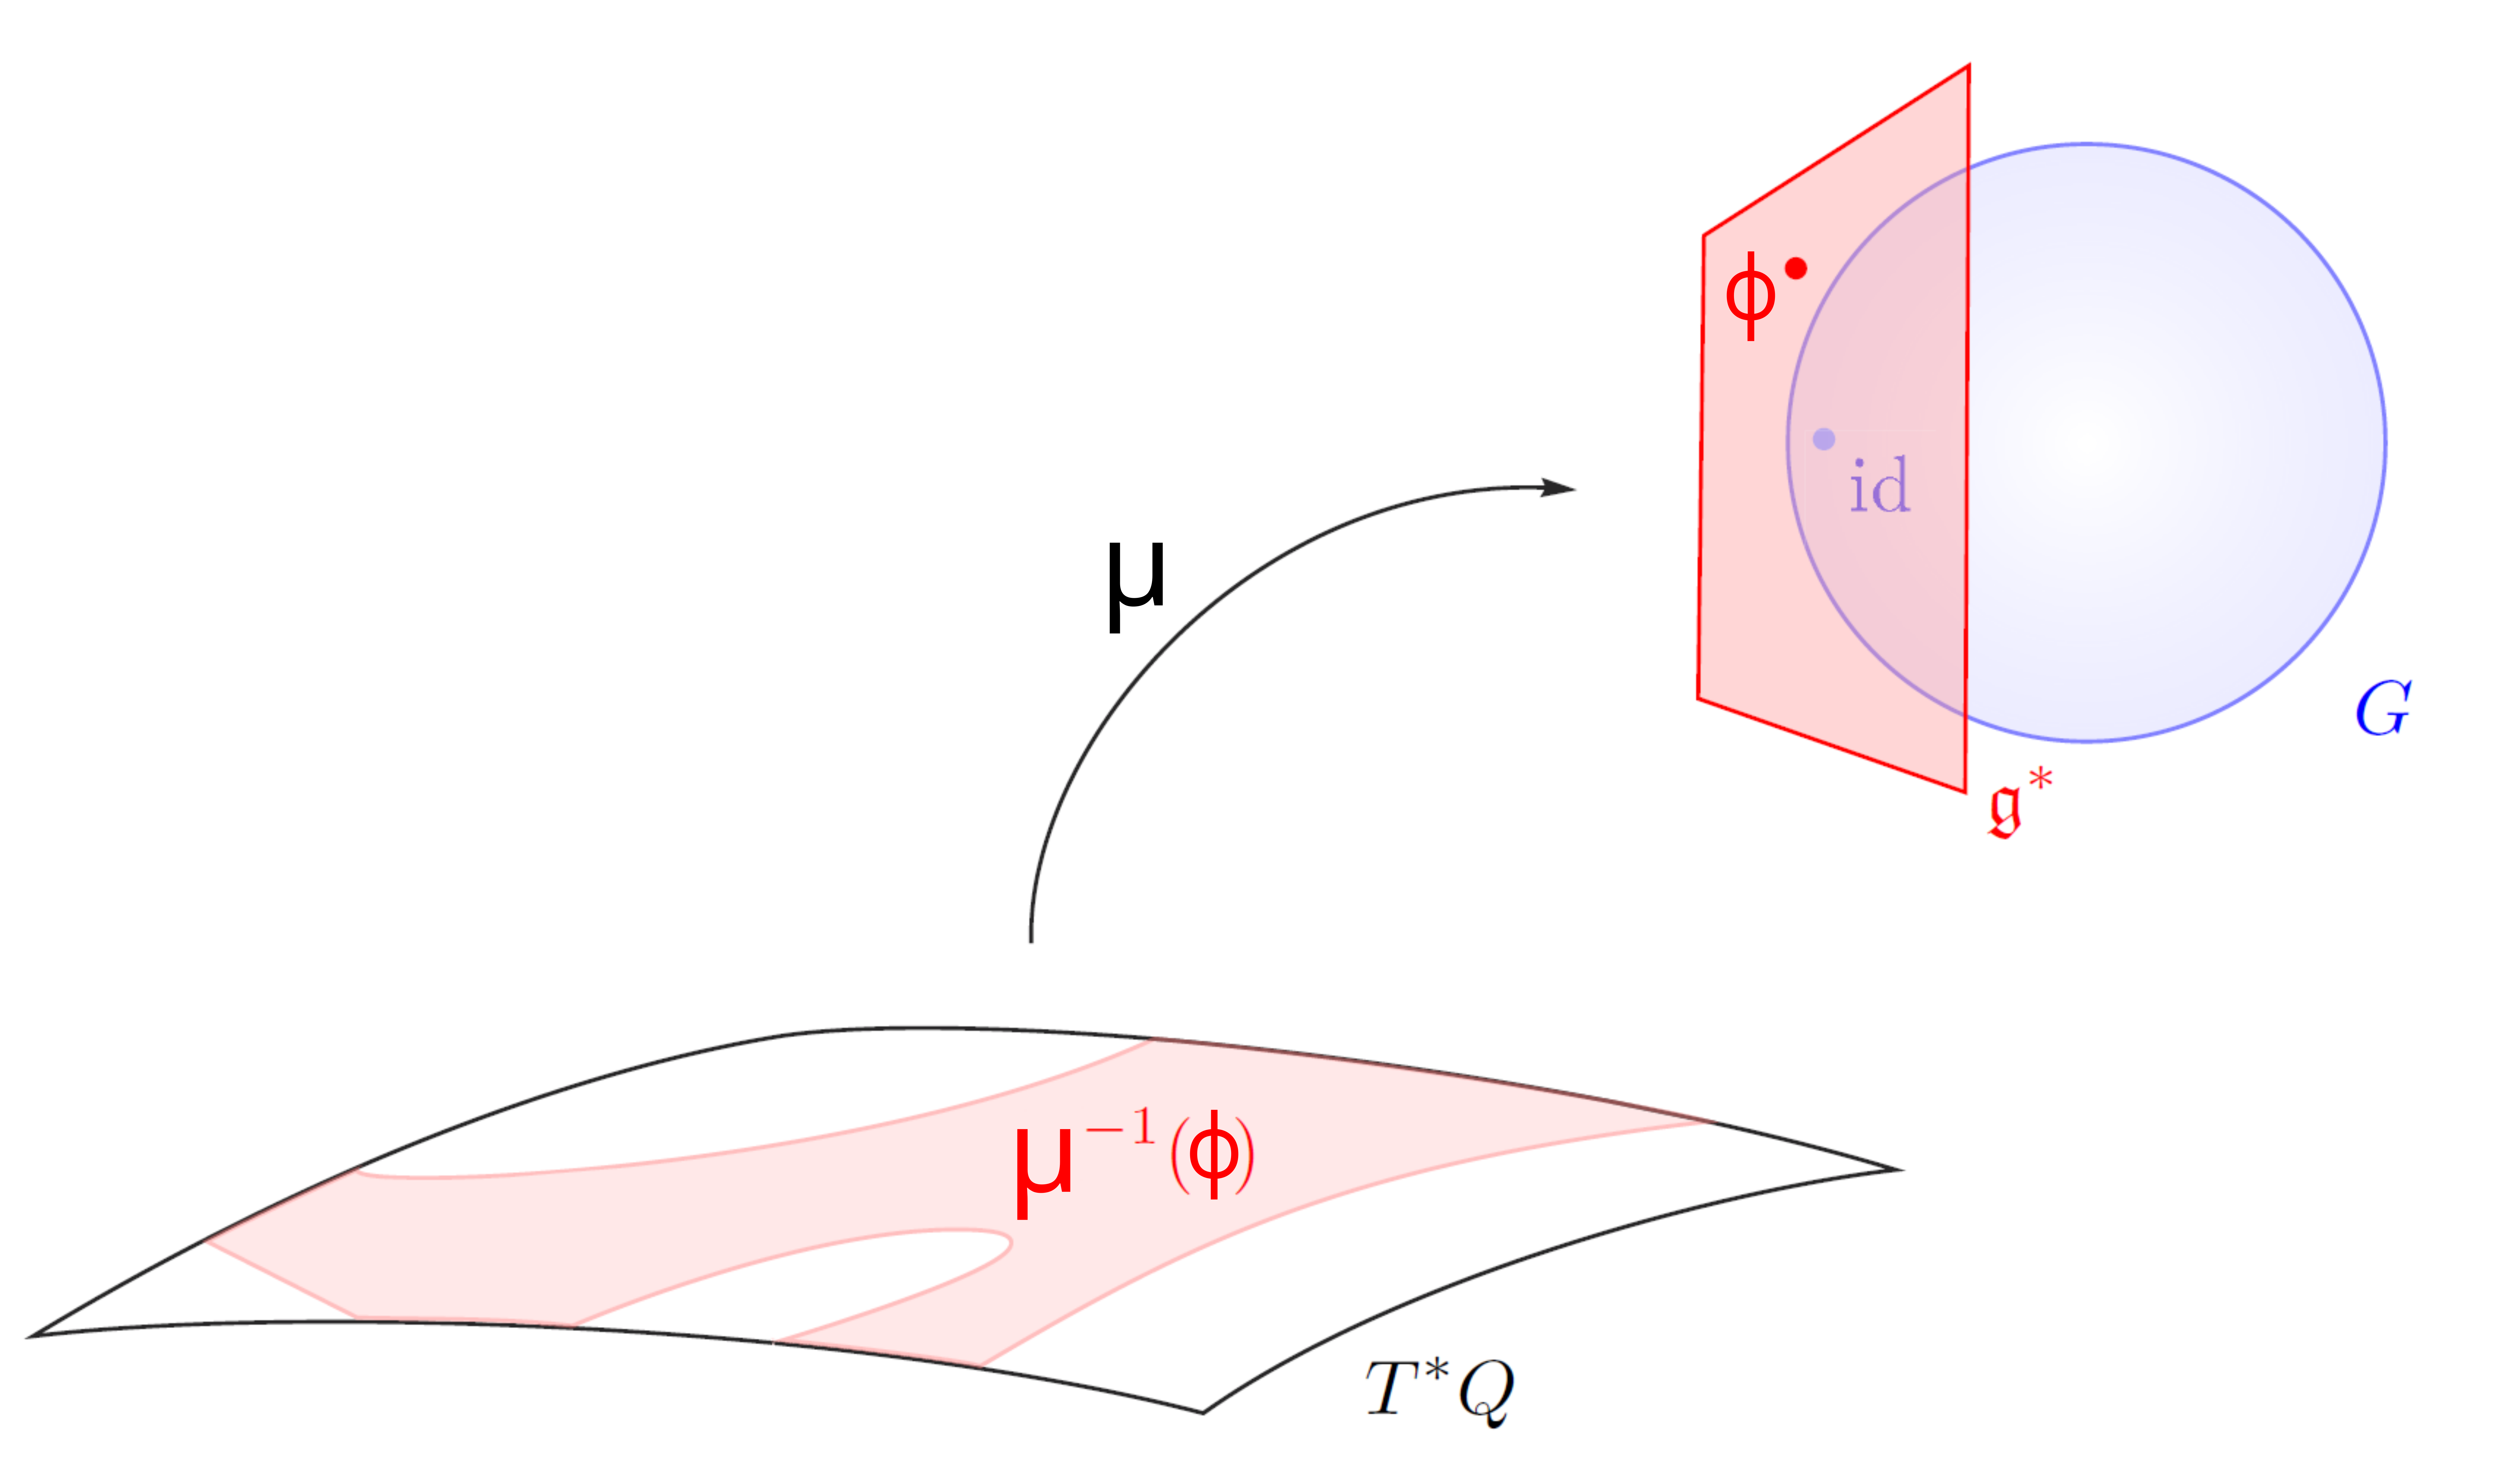
\includegraphics[width=\textwidth]{Pictures/Reduction} 
  	\end{column}
	\end{columns}			
\end{frame}
%------------------------------------------------------------------------------------------------



%---------------------------------------------------------------------------------------------------------------------------------------------------
\begin{frame}{Research proposal context: (multi)symplectic reduction}
	\textbf{\color{UniGreen}Symplectic reduction:}~~
	Procedure associating to any (suitably regular) pair of symplectic manifold and Hamiltonian action another symplectic manifold of smaller dimension.
	\vfill
	\pause
	\begin{thmblock}[Marsden-Weinstein reduction]
		\vspace{-.4em}
		\begin{tabular}{l p{12cm}}
		    Given: & $(M,\omega)$ symplectic
		    \\
		    & $G\curvearrowright M$ symplectic with equivariant momap. $J:M\to \mathfrak{g}^*$
		    \\[.2em]
		    Assume: & $\mu \in \mathfrak{g}^*$ regular value of $J$ 
		    \qquad\quad \footnotesize \textcolor{gray}{($\Rightarrow$ $J^{-1}(\mu)\hookrightarrow M$ smooth embedding)}
		    \\
			& $G_\mu\action J^{-1}(\mu)$ free and proper
			\quad \footnotesize \textcolor{gray}{($\Rightarrow$ $J^{-1}(\mu)/G_\mu$ smooth manifold)}
			\\[.4em]
			Then: & $\exists!$ symplectic structure $\omega_\mu$ in $M_\mu:= J^{-1}(\mu)/G_\mu$ \\
			& s.t. $\pi^\ast \omega_\mu = j^\ast \omega$ with $j:M_\mu \hookrightarrow M$ and $\pi:M\twoheadrightarrow M_\mu$
		\end{tabular}
		\vspace{-.4em}
	\end{thmblock}
	%
	\vfill
	\pause
	\begin{columns}
		\begin{column}{0.40\textwidth}
			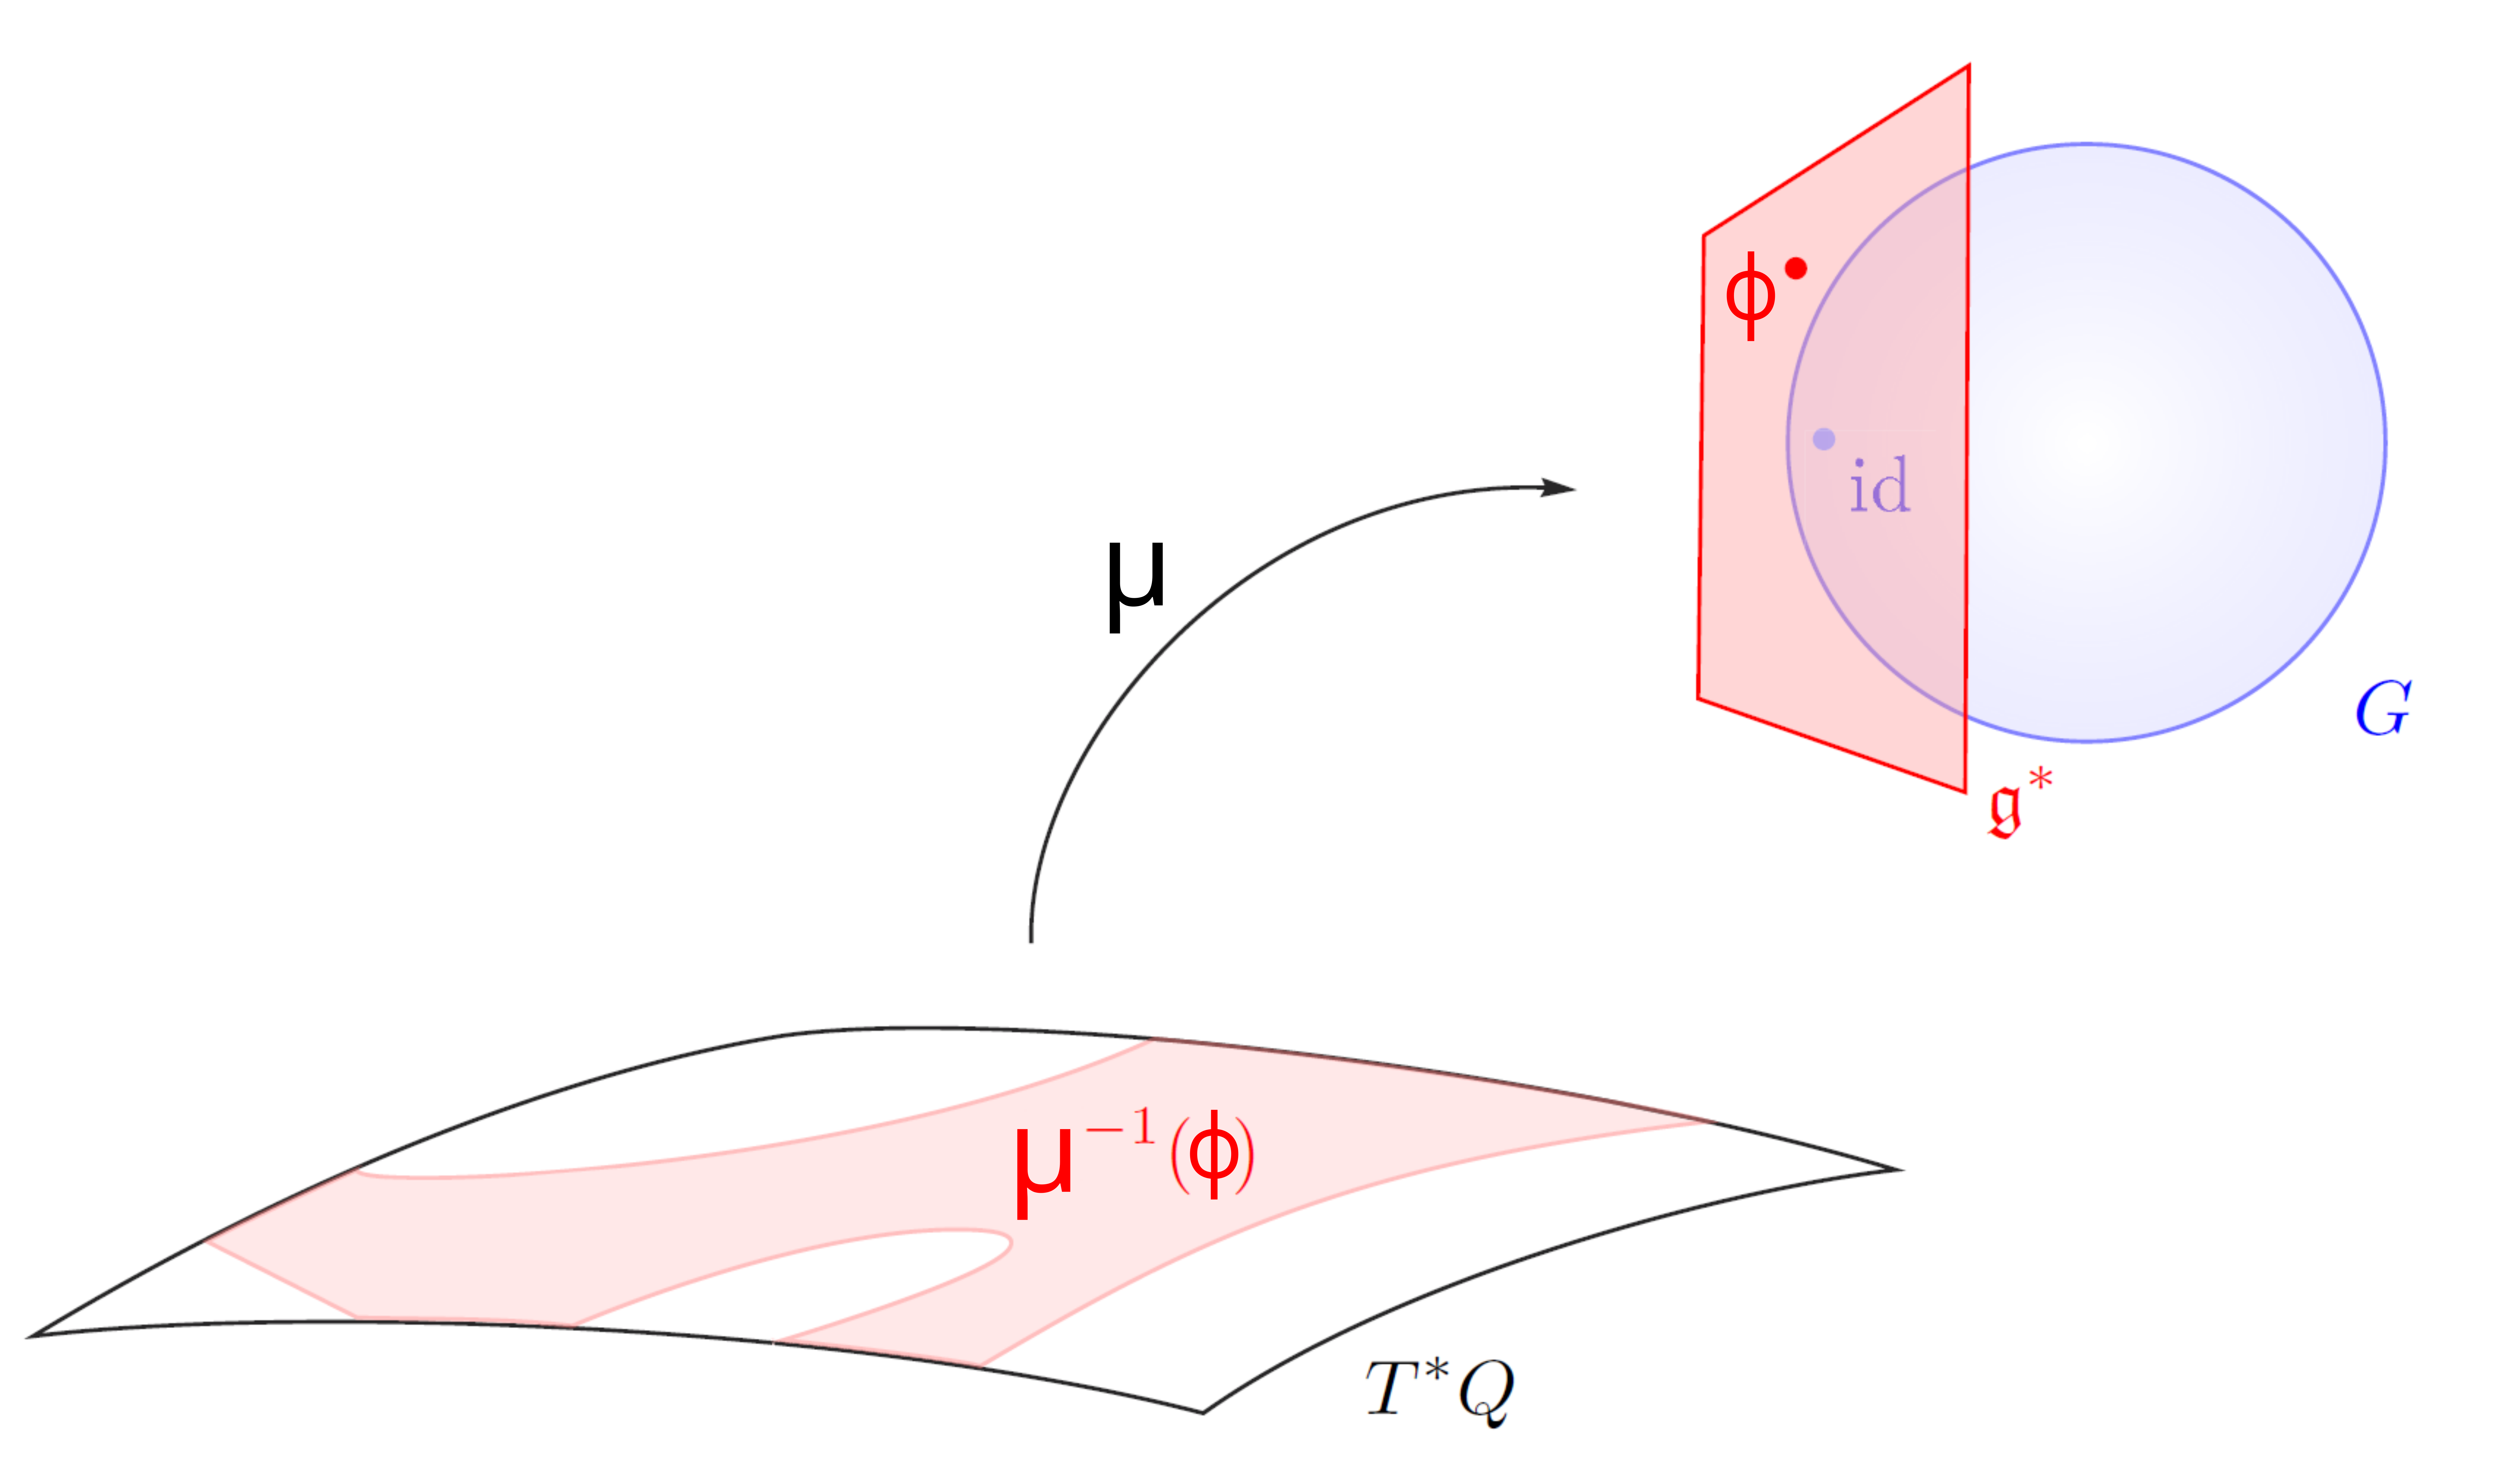
\includegraphics[width=\textwidth]{Pictures/Reduction}
		\end{column}	
		
		\begin{column}{0.6\textwidth}
				\textbf{\color{UniGreen}In mechanics:}~~
			it embodies the process of restricting the dynamics of the system to the level sets of the conserved quantities pertaining to the symmetry group.		
			\\
			\color{gray}\small( e.g. restricting to studying a point-like particle in a central potential by studying it in radial coordinates only)
		\end{column}	
	\end{columns}	


\end{frame}
%---------------------------------------------------------------------------------------------------------------------------------------------------

%-------------------------------------------------------------------------------------------------------------------------------------------------
\begin{frame}[fragile,shrink]{Homotopy co-moment maps \emph{(Callies, Fregier, Rogers, Zambon)}}
	\begin{columns}
		\begin{column}{.625\linewidth}	
			HCMM is an $L_\infty$-morphism  $\quad(f):\mathfrak{g}\to L_\infty(M,\omega)$
			\\[.5em]
			 lifting the  infinitesimal action $\quad v:\mathfrak{g}\to \mathfrak{X}(M)$
		\end{column}
		\begin{column}{.325\linewidth}	
			\begin{displaymath}
				\begin{tikzcd}[column sep = large]
					& L_{\infty}(M,\omega) \ar[d,"\mathscr{v}"]
					\\
					\mathfrak{g} \ar[ur,dashed,"(f)"]\ar[r,"v"']& \mathfrak{X}(M)
				\end{tikzcd}	
			\end{displaymath}		
		\end{column}
	\end{columns}
	\pause
	\begin{lemblock}[HCMM unfolded  \cite{Callies2016}]
			%
			HCMM is a sequence of (graded-skew) multilinear maps:
			\begin{displaymath}
				(f)  = \big\lbrace f_k: \; \Lambda^k{\mathfrak g} \to L_{k-1} \subseteq \Omega^{n-k} 
				\;\big\vert\; 0\leq k \leq n+1  \big\rbrace
			\end{displaymath}
			%
			\vspace{-.5em}	
			\includestandalone[width=0.9\textwidth]{Pictures/Frame_HCMM}
			
			\vspace{-1em}		
			\emph{fulfilling:}%\emph{such that:}
			\begin{itemize}
				\item<2-> $f_0 = 0 $, $f_{n+1} = 0$
				\item<3-> $d f_k (p) = f_{k-1} (\partial p)  - (-1)^{\frac{k(k+1)}{2}} \iota(v_p) \omega 
				\qquad\scriptstyle \forall p \in \Lambda^k(\mathfrak{g}),\; \forall k=1,\dots n+1$
			\end{itemize}
		\end{lemblock}

	\begin{tamblock}
	 Practically a HCMM is given by several multilinear maps
	 \begin{displaymath}
	 	f_i = \Lambda^i \mathfrak{g} \to L_{i-1}
	 \end{displaymath}
	 satisfying:
	 \begin{enumerate}
	 	\item $ d f_1(\xi) = - \iota_{v_\xi} \omega$
	 	\item $\sum ...$
	 \end{enumerate}
	\end{tamblock}


\end{frame}
\note[itemize]{
	%\item 		Consider:  $v:\mathfrak g\to \mathfrak X(M)$  a Lie algebra morphism  s.t. $\mathcal{L}_{v_x}\omega=0 \quad  \forall x\in\mathfrak g$ (i.e infinitesimal multisymplectic Lie algebra action $\mathfrak{g}\circlearrowleft (M,\omega)$)
	\item More conceptually, a comoment is an $L_\infty$-morphism $(f):\mathfrak{g}\to L_\infty(M,\omega)$ lifting the action $v:\mathfrak{g}\to \mathfrak{X}(M)$, 
i.e. making the diagram commute in the $L_\infty$-algebras category.
	\item The vertical arrow is the trivial $L_\infty$-extension of the function mapping any Hamiltonian form to the unique corresponding Hamiltonian vector field (an it is zero elsewhere)
		\\
		(Note that any Lie algebra can be seen as an $L_\infty$-algebra concentrated in degree $0$, therefore any $L_\infty$-morphism $L\to\mathfrak{g}$ is simply given by a linear map $L_0 \to \mathfrak{g}$ preserving the binary brackets.)
	\item We will make use of an explicit version of this definition which is expressed by the lemma.
	 Practically speaking, a HCMM is given by several multilinear maps ...
	 \item In the equation we have tacitly set $\Lambda^{-1}(M) = 0$
	 %\item Notation: \qquad $\partial =$ Chevalley-Eilenberg boundary operator.
	%\item Notice that a HCMM pertains to an "infinitesimal" action of ${\mathfrak g}$ on $M$ with ${\mathfrak g}$ being the Lie algebra of a generic Lie group $G$, acting on $M$ by $\omega$-preserving vector fields.
		\item (Notation) $ p = \xi_1 \wedge \xi_2 \wedge \dots \wedge \xi_k$, 
			then $v_p = v_1 \wedge v_2 \wedge \dots \wedge v_k$ 
			where $v_i \equiv v_{\xi_i}$ are the fundamental vector fields associated to the action $G \circlearrowright M$.
	%	\item (Notation) $\iota(v_p) \omega = \iota(v_k)\dots\iota(v_1) \omega$
	%	\item $\varsigma(k) := - (-1)^{\frac{k(k+1)}{2}}$ 
		\item (Notation) $(\iota^{k}_{\mathfrak{g}}\omega)(p):= \iota(v_p) \omega = \iota(v_k)\dots\iota(v_1) \omega$
		\item $\partial \equiv \partial_k:  \Lambda^{k} {\mathfrak g} \to \Lambda^{k-1} {\mathfrak g}$  is the usual Eilenberg-Chevalley complex boundary operator (see appendix, pag: \ref{frame:CE-complex});
%		\item The definition tells us that the {\it closed} forms
%			$$\mu_k := f_{k-1} (\partial p) +  \varsigma(k) \iota(v_p) \omega 	$$
%			must actually be {\it exact}, with potential $-f_k(p)$.  	
		\item The last equation tells us that an HCMM is not a chain complex morphism but is rather a chain complex homotopy between 0 and the multicontraction $\alpha=(\iota^{k}_{\mathfrak{g}}\omega)$ (see next slide).
		is a chain map by lemma 2.18 \cite{Ryvkin2016}).
}
%---------------------------------------------------------------------------------------------------------------------------------

%-------------------------------------------------------------------------------------------------------------------------------------------------
\begin{frame}[t]{Symmetries in \textbf{multisymplectic geometry}}
	Consider a Lie algebra action $v:\mathfrak{g} \to \mathfrak{X}(M)$  preserving the $n$-plectic form $\omega$,
	\vfill

	\vspace{-1em}
	\begin{columns}[T]
		\setlength{\belowdisplayskip}{5pt}
		\begin{column}{.50\linewidth}
			%
			\centering \it
			\onslide<2->{
				$-$ symplectic case $-$
				\begin{defblock}[Comoment map pertaining to $v$]
					Lie algebra morphism
					$$ f: \mathfrak{g} \to C^\infty(M) $$
					such that
					$$ d~f (x) = -\iota_{v_x} \omega \qquad \forall x \in \mathfrak{g}~.$$
				\end{defblock}
			}
		\end{column}	
		%
		\onslide<2->{\vrule{}}
		%
		\begin{column}{.50\linewidth}
			\centering \it
			\onslide<3->{			
				$-$ $n$-plectic case $-$
				\begin{defblock}[Homotopy comoment map \tiny (HCMM)]
					$L_\infty$-morphism 
					$$ (f_k) : \mathfrak{g} \to L_\infty (M,\omega)$$
					such that
					$$ d~f_1(x) = -\iota_{v_x} \omega \qquad \forall x \in \mathfrak{g}~.$$
				\end{defblock}	
			}
		\end{column}	
	\end{columns}	
	%
	\pause
	\vfill
	\centering 
	\onslide<4->{\textbf{-- Conserved quantities --}}
	%
	\vspace{-.5em}
	\begin{columns}[T]
		\setlength{\belowdisplayskip}{5pt}
		\begin{column}{.50\linewidth}
			%
			\centering \it
			\onslide<4->{
			\begin{propblock}[Noether Theorem]
				\small Fixed $H\in C^\infty_{\text{Ham}}(M)$ ($\mathfrak{g}$-invariant) ,
				$$\mathcal{L}_{v_H} f(x) = 0 \qquad \forall x \in \mathfrak{g}$$
			\end{propblock}
			}
		\end{column}	
		%
		\onslide<5->{\vrule{}}
		%
		\begin{column}{.50\linewidth}
			\centering \it
			\onslide<5->{			
			\begin{propblock}[RWZ16 Theorem]
				\small Fixed $H\in \Omega^{n-1}_{\text{Ham}}(M)$ ($\mathfrak{g}$-invariant),
				$$\mathcal{L}_{v_H} f_k(p) \in B^k(M) \qquad \forall p \in Z_k(\mathfrak{g})$$			
			\end{propblock}
			}
		\end{column}	
	\end{columns}		
\end{frame}
%-------------------------------------------------------------------------------------------------------------------------------------------------


\end{document}

%-------------------------------------------------------------------------------------------------------------------------------------------------
\section{Algebraic singular reduction}
\checkpoint	
%-------------------------------------------------------------------------------------------------------------------------------------------------
	%- HandOut Flag -----------------------------------------------------------------------------------------
\makeatletter
\@ifundefined{ifHandout}{%
  \expandafter\newif\csname ifHandout\endcsname
}{}
\makeatother

%- D0cum3nt ----------------------------------------------------------------------------------------------
\documentclass[beamer,10pt]{standalone}   
%\documentclass[beamer,10pt,handout]{standalone}  \Handouttrue  

\ifHandout
	\setbeameroption{show notes} %print notes   
\fi

	
%- Packages ----------------------------------------------------------------------------------------------
\usepackage{custom-style}
\usepackage{math}
\usetikzlibrary{positioning}
\usepackage{multicol}
\usepackage{xfrac}

%--Beamer Style-----------------------------------------------------------------------------------------------
\usetheme{toninus}
\usepackage{animate}
\usetikzlibrary{positioning, arrows}
\usetikzlibrary{shapes}

\renewcommand{\action}{\curvearrowright} 
\makeatletter
\def\blfootnote{\gdef\@thefnmark{}\@footnotetext}
\makeatother

\begin{document}

%-------------------------------------------------------------------------------------------------------------------------------------------------
\subsection{Symplectic singular reduction}
\begin{frame}{Singular reduction schemes}
	\begin{block}{The gist of singular reduction}
 		\begin{itemize}
 			\item[-] when $\mu$ is singular (i.e. $\mu^{-1}(0)$ is not a mfd.), the (geometrically) reduced space may not exist.
 			\item[-] a \emph{singular reduction scheme} is a procedure to construct a "reduced" algebra of observable out of the given data
 			\item[-] such that it corresponds to the algebra of observable of the reduced manifold in the regular case.
 		\end{itemize}
	\end{block}
 
	\begin{thmblock}[Sniatycki-Weinstein reduction \cite{SniatyckiWeinstein83}]
		\vspace{-.4em}\hspace{-1em}
		\begin{tabular}{l p{14cm}}
		    Given: & $(M,\omega)$ symplectic
		    \\
		    & $G\curvearrowright M$ symplectic with equivariant momap. $\mu:M\to \mathfrak{g}^*$
			\\[.4em]
			Then: & 
			$\displaystyle \left[\sfrac{C^\infty(M)}{I_\mu}\right]^G$
			admits a Poisson algebra structure 
			\blfootnote{$I_\mu$ = associative ideal generated by $\widetilde{\mu}(\g)$}			
			\\
			& it agrees with the M--W reduction in the regular case.		
		\end{tabular}
		\vspace{-.4em}
	\end{thmblock}
 

\end{frame}
\note[itemize]{
 \item
}
%-------------------------------------------------------------------------------------------------------------------------------------------------

%-------------------------------------------------------------------------------------------------------------------------------------------------
\begin{frame}[shrink]{Smooth objects on a singular set}
	Consider $N$ closed subset of $M$.
	\vfill
	\pause
	\begin{defblock}
	 $I_N$ = ideal of smooth functions vanishing over $N$.
	\end{defblock}
	\vfill
	\pause

	\begin{columns}[T]
		\setlength{\belowdisplayskip}{5pt}
		\begin{column}{.65\linewidth}
			%
			\centering \it
				\begin{defblock}[v.f tangent to $N$]
					\begin{displaymath}
						\X_N(M):=
						\left\lbrace
							v \in \X(M)
						~\Big\vert~
							\L_v(I_N) \subseteq I_N
						\right\rbrace
					\end{displaymath}
				\end{defblock}
				\begin{defblock}[v.f vanishing on $N$]
					\begin{displaymath}
						I_\X(N):=
						\left\lbrace
							v \in \X(M)
						~\Big\vert~
							\L_v(C^\infty(M)) \subseteq I_N
						\right\rbrace
					\end{displaymath}				
				\end{defblock}				
		\end{column}	
		%
		%
		\begin{column}{.35\linewidth}
			\centering 
			\includestandalone[width=0.9\textwidth]{Pictures/Figure_VfTangentN}			
		\end{column}	
	\end{columns}			
	%	

				%

				%	
		\begin{tcolorbox}[
		enhanced,frame hidden,borderline={0.5pt}{0pt}{blue},
		arc=5pt,colback=white,
		colbacktitle=white,]
			\color{blue}{\textbf{Lem}:} If $N$ is smoothly embedded,  $\X(N)\cong \dfrac{X_N(M)}{I_\X}$.
		\end{tcolorbox}


		\begin{defblock}[Differential form vanishing on $N$]
			\begin{displaymath}
				I_{\Omega(N)}:=
				\left\lbrace
					\alpha\in\Omega^k(M
				~\left\vert~
					\begin{array}{l r}
						k\geq 0,~		\\		
						\alpha(u_1,\ldots,u_k) \in I_N & \forall u_i \in\X_N(M)
					\end{array}
				\right\rbrace\right.
			\end{displaymath}
		\end{defblock}

\end{frame}
\note[itemize]{
 \item $N$ is not a submanifold in general. An example is $N=\mu^{-1}(0)$ for a certain smooth map $N$.
 \item observe that if $N$ is a smooth embedded submanifold, one has that $\X(N)\cong \frac{X_N(M)}{I_\X}$  

}
%-------------------------------------------------------------------------------------------------------------------------------------------------



%-------------------------------------------------------------------------------------------------------------------------------------------------
\subsection{Multisymplectic singular reduction}
\begin{frame}{Reducible smooth objects}
	Consider $\g \action M$ by vector field tangent to $N$ \hfill($\underline{\g}\subseteq \X_N(M)$)
	
	\begin{defblock}[Reducible v.fields w.r.t. $\g\action M$]
			\begin{displaymath}
				\X(M)_{[N]} :=
				\left\lbrace
					v \in \X(M)
				~\left\vert~
					\begin{array}{l}
						\L_v (I_N) \subseteq I_N	\\		
						\L_v (\X_g) \subseteq \X_g + I_\X
					\end{array}
				\right\rbrace\right.
			\end{displaymath}
			\blfootnote{
			 $\X_g$ = $C^\infty(M)$-module generated by the fundamental distribution.
			}	

	\end{defblock}	
	
	\begin{defblock}[Reducible forms w.r.t. $\g\action M$]
		\begin{displaymath}
			\Omega(M)_{[N]} :=
			\left\lbrace
				\alpha \in \Omega(M)
			~\left\vert~
				\begin{array}{l r}
					\L_\underline{\xi} \,\alpha \in I_{\Omega(N)}	\\		
					\iota_\underline{\xi} \,\alpha \in I_{\Omega(N)}	& \forall \xi \in \g				\end{array}
			\right\rbrace\right.
		\end{displaymath}	
	\end{defblock}	

	\begin{defblock}[Reducible Hamiltonian forms w.r.t. $\g\action M$]
		\begin{displaymath}
			(\Omega(M)_{ham}^{n-1})_{[N]} :=
			\left\lbrace
				\alpha \in \Omega(M)_{ham}^{n-1}
			~\left\vert~
				\begin{array}{l r}
					\alpha \text{ is a reducible form} \\
					\vHam_\alpha \text{ is a reducible v.field}
				\end{array}
			\right\rbrace\right.
		\end{displaymath}	
	\end{defblock}		

	
\end{frame}
\note[itemize]{
 \item $\g\action M$ by vector field tangent to $N$ means that $\underline{\xi}\in\X_n(M) \forall \xi \in \g$
 \item Spelling out the definition: reducible vector fields are 
 \\i) v.f. tangent to N 
 \\ii) such that their commutator with any $\underline{\xi}$ lies in $\X_\g$ along $N$.
 \item more algebraically, they stabilize both $I_N$ and $\X_g + I_\X$.
 \item observe that $\L_v I_\X \subseteq I_\X$ since , $\forall u \in I_\X$ $\forall f \in C^\infty(M)$ one has\\
 $(\L_v u) f = \L_{[v,u]} f = \L_v\L_u f - \L_u\L_v f \in I_N$
 \item
}
%-------------------------------------------------------------------------------------------------------------------------------------------------

%-------------------------------------------------------------------------------------------------------------------------------------------------
\begin{frame}{Singular reduction}
	\begin{defpropblock}[Reducible $L_\infty$-observables]
		Is the {\color{blue!70!black}$L_\infty$-subalgebra} of $L_\infty(M,\omega)$ given by
		\begin{displaymath}
			L_\infty(M,\omega)_{[N]}^k :=
			\begin{cases}
				\Omega^{n-1-k}(M)_{[N]} 
				\qquad\text{\color{gray}\small (reducible forms) }
				& \text{if } n-1\leq k < 0 \\
				(\Omega(M)_{ham}^{n-1})_{[N]} 
				\quad
				\text{\color{gray}\small (reducible hamiltonians) }
				& \text{if } k = 0 \\
				0 & \text{if } k > 0
			\end{cases}
		\end{displaymath}
	\end{defpropblock}

	\begin{defpropblock}[Vanishing $L_\infty$-observables]
		Is the {\color{blue!70!black}$L_\infty$-ideal} of $L_\infty(M,\omega)_{[N]}$ given by
		\begin{displaymath}
			I_{L_\infty(M,\omega)} :=
			\left\lbrace
				\alpha \in L_\infty(M,\omega)_{[N]}
			~\left\vert~
				\begin{array}{l l}
					\alpha(v_1,\dots,v_k) \in I_N  \quad \forall v_i \in \X_N &
					\text{if}~ \alpha \in \Omega^k \\
					\vHam_\alpha \in \X_\g + I_\X &
					\text{if}~ \alpha \in \Omega^{n-1}
				\end{array}
			\right\rbrace\right.
		\end{displaymath}
	\end{defpropblock}

	\begin{defblock}[Reduced $L_\infty$-algebra of observables]
		Is the $L_\infty$-quotient : \quad
		$\dfrac{L_\infty(M,\omega)_{[N]}^k}{I_{L_\infty(M,\omega)}}$
	\end{defblock}

\end{frame}
\note[itemize]{
 \item
}
%-------------------------------------------------------------------------------------------------------------------------------------------------



\end{document}






%------------------------------------------------------------------------------------------------
% APPENDIX
%------------------------------------------------------------------------------------------------
\appendix
%-------------------------------------------------------------------------------------------------------------------------------------------------
\section{Complementary Material}
	%+----------------------------------------------------------------------------+
%| SLIDES: 
%| Chapter: Complementary material - details on eventual questions
%| Author: Antonio miti
%| Event: PHD preliminary Defence
%+----------------------------------------------------------------------------+

%- HandOut Flag -----------------------------------------------------------------------------------------
\newif\ifHandout

%- D0cum3nt ----------------------------------------------------------------------------------------------
\documentclass[beamer,10pt]{standalone}   
%\documentclass[beamer,10pt,handout]{standalone}  \Handouttrue  

%- HandOut Flag -----------------------------------------------------------------------------------------
\ifHandout
	\setbeameroption{show notes} %print notes   
\fi

	
%- Packages ----------------------------------------------------------------------------------------------
\usepackage{custom-style}

%--Beamer Style-----------------------------------------------------------------------------------------------
\usetheme{toninus}



\providecommand{\blank}{\text{\textvisiblespace}}


\newcommand{\subsectiontitle}{
  \begin{frame}
  \vfill
  \centering
  \begin{beamercolorbox}[sep=8pt,center,shadow=true,rounded=true]{title}
    \usebeamerfont{title}\insertsectionhead\par%
    \usebeamerfont{title}\insertsubsectionhead\par%
  \end{beamercolorbox}
  \vfill
  \end{frame}
}

\providecommand{\blank}{\text{\textvisiblespace}}




%---------------------------------------------------------------------------------------------------------------------------------------------------
%- D0cum3nt ----------------------------------------------------------------------------------------------------------------------------------
\begin{document}
%------------------------------------------------------------------------------------------------

%##################################################################################
\begin{frame}
	\begin{center}
	\Huge\emph{Supplementary Material}
	\end{center}
\end{frame}
\note[itemize]{
	\item
}
\addtocounter{framenumber}{-1}
%##################################################################################



%------------------------------------------------------------------------------------------------
\begin{frame}[fragile]{MS geometry and classical field mechanics}\label{Frame:Ms-Field-Mechanics}
		Consider a smooth manifold $Y$,
		\begin{columns}
			\hfill
			\begin{column}{.5\linewidth}
				\emph{Multicotangent bundle} $\bigwedge = \bigwedge^n T^\ast Y$\\
				is naturally $n$-plectic
			\end{column}
			\begin{column}{.4\linewidth}
				\[
				\begin{tikzcd}
					\Lambda \ar[d,"\pi"'] & T \Lambda \ar[d,"T \pi"] \ar[l] \\
					Y								& T Y \ar[l]
				\end{tikzcd}	
				\]
			\end{column}
		\end{columns}
	\pause
	\begin{defblock}[Tautological $n$-form]
		$\theta \in \Omega^n(\Lambda)$ such that:
		\begin{displaymath}
		\begin{split}
			\left[ \iota_{u_1 \wedge \ldots \wedge u_n} \theta \right]_\eta 
			&= \iota_{(T \pi)_\ast u_1 \wedge \ldots \wedge (T \pi)_\ast u_n} \eta \\
			&= \iota_{u_1 \wedge \ldots \wedge u_n} \pi^\ast \eta 
			\qquad \qquad \forall \eta \in \Lambda \, , \: \forall u_i \in T_\eta \Lambda 		
		\end{split}
		\end{displaymath}
	\end{defblock}
	\vfill
	\begin{columns}
		\begin{column}{.6\linewidth}
			\begin{defblock}[Tautological (multisymplectic) (n+1)-form]
				$$\omega := d \theta$$
			\end{defblock}
		\end{column}
		\begin{column}{.4\linewidth}
		 	\begin{claimblock}$\omega$ is not degenerate.\end{claimblock}	
		\end{column}
	\end{columns}	
	\pause
	\begin{keywordblock}
		\begin{tabular}{|c|c|c|}
			\hline 
			point-particles mechanics & $\rightsquigarrow$ & classical fields mechanics \\
			%(finite discrete DOF) & & (finite dimensional continuous DOF) \\
			\hline 
			symplectic & $\rightsquigarrow$ & multisymplectic \\ 
			\hline 
			Observables (Poisson) algebra & $\rightsquigarrow$ & Observables $L-\infty$ algebra
			 \\ 
			\hline 
			Co-moment map & $\rightsquigarrow$ & Homotopy co-momentum map \\ 
			\hline 
		\end{tabular} 
	\end{keywordblock}

	
\end{frame}
\note[itemize]{
	\item This example is significant from the perspective of geometric classical field theory:
		\begin{displaymath}
			\frac{\text{classical mechanics}}{\text{symplectic geo.}} =
			\frac{\text{classical field mechanics}}{\text{multisymplectic geo.}}
		\end{displaymath}
	\item Multicotangent bundle is the \emph{Higher analogue} of the cotangent bundle.
	(but it is not yet the analogue of a \emph{phase space}.)
\item The multiphase space is the sub-bundle of $n$-forms vanishing when contracted with 2 vertical fields.
  	\item The reason why this sub-bundle has a particular role is that it can be proved to be isomorphic to a suitable dual of the first Jet bundle.
  	\item For further details see Gotay et al. \href{https://arxiv.org/abs/physics/9801019}{arXiv:physics/9801019}. For a pictorial representation of all the structures involved in the geometric mechanics of I order classical field theories see appendix, pag: \ref{frame:Gimmsy}.
}
%------------------------------------------------------------------------------------------------	
	

\begin{frame}[fragile,shrink]{Unwrapping the \emph{higher Jacobi equations}}\label{Frame:unwapping-Jacobi}
\underline{Slogan:} \emph{Jacobi identity satisfied up to an higher coherent homotopy}
		%
		\vspace{1.5em}
		\begin{columns}[c]
			\hfill
			\begin{column}{0.5\linewidth}
				Higher Jacobi implies:
				\begin{itemize}  \setlength\itemsep{1em}
					\item Underlying chain-complex $(L,\mu_1)$ with differential $d=\mu_1$;
					\item \color{red} $\mu_2 = [\cdot,\cdot]$ is a chain map $L^{\otimes 2} \to L$;
					\item \color{green!20!black}$\mu_3=j(\cdot,\cdot,\cdot)$ is a chain homotopy 
						$\mu_2\circ\mu_2 \Rightarrow 0$;
						\\ i.e. between the usual Jacobiator ${[[\cdot,\cdot],\cdot]} \circ P_{\text{unsh}}$ and the $0$ map 
					\item \color{purple}higher analogues...	
					\\ e.g. $\mu_4$, is a second order chain-homotopy between the two chain homotopies  ${[j(\cdot,\cdot ,\cdot]),\cdot]}\circ P_{\text{unsh}}$ and ${j([\cdot , \cdot],\cdot,\cdot)}\circ P_{\text{unsh}}$
				\end{itemize}
			\end{column}
			\begin{column}{0.45\linewidth}
				\includestandalone[width=0.9\linewidth]{Pictures/Figure_Linfinity_diagram}
			\end{column}	
		\end{columns}	
		\vspace{1.5em}
		Notation: $P_{\text{unsh}}$ = sum on all the possibile unshuffled permutation.

\end{frame}
\note[itemize]{
  \item Regarding any $l_k$ as a tree with $k$ entries and 1 output, the $k$-th generalized Jacobi equation is produced summing all the possible way to obtain a $k+1$-ary tree by composing two other trees (not more then two!).
  \item Can be regarded as
  	\begin{displaymath}
  		\sum_{i+j = k} l_j \circ ( l_j \otimes \mathbb{I}) \circ P_{\text{unsh}}
  	\end{displaymath}
  	Where $P_{\text{unsh}} : L^{\otimes(k-1)} \rightarrow L^{\otimes(k-1)} $ is the $(i,j)$-unshuffolator.
  	\\(you consider only unshuffles to avoid the redundancies given by the fact that any $l_i$ has fixed symmetry.
  \item Examples of unshuffles: \\
  \begin{displaymath}
  \begin{split}
  	(12)(3)\quad(13)(2)\quad(23)(1)\\
  	(123)(4)\quad(234)(1)\quad(134)(2)\quad(124)(3)\\
  	(12)(34)\quad(23)(14)\quad(13)(24)\quad(14)(23)\quad(24)(13)
  \end{split}
  \end{displaymath}
	\item When regarding the L$\infty$ structure as a chain complex with homotopies you get a neat intepretation of the Jacobi identity at the price that \emph{graded skew-symmetry} definition is more obscure than in the presentation with graded vector spaces.
}
%------------------------------------------------------------------------------------------------



%-------------------------------------------------------------------------------------------------------------------------------------------------
\begin{frame}[t]{Symmetries in \textbf{multisymplectic geometry}}
	Consider a Lie algebra action $v:\mathfrak{g} \to \mathfrak{X}(M)$  preserving the $n$-plectic form $\omega$,
	\vfill

	\vspace{-1em}
	\begin{columns}[T]
		\setlength{\belowdisplayskip}{5pt}
		\begin{column}{.50\linewidth}
			%
			\centering \it
			\onslide<2->{
				$-$ symplectic case $-$
				\begin{defblock}[Comoment map pertaining to $v$]
					Lie algebra morphism
					$$ f: \mathfrak{g} \to C^\infty(M) $$
					such that
					$$ d~f (x) = -\iota_{v_x} \omega \qquad \forall x \in \mathfrak{g}~.$$
				\end{defblock}
			}
		\end{column}	
		%
		\onslide<2->{\vrule{}}
		%
		\begin{column}{.50\linewidth}
			\centering \it
			\onslide<3->{			
				$-$ $n$-plectic case $-$
				\begin{defblock}[Homotopy comoment map \tiny (HCMM)]
					$L_\infty$-morphism 
					$$ (f_k) : \mathfrak{g} \to L_\infty (M,\omega)$$
					such that
					$$ d~f_1(x) = -\iota_{v_x} \omega \qquad \forall x \in \mathfrak{g}~.$$
				\end{defblock}	
			}
		\end{column}	
	\end{columns}	
	%
	\pause
	\vfill
	\centering 
	\onslide<4->{\textbf{-- Conserved quantities --}}
	%
	\vspace{-.5em}
	\begin{columns}[T]
		\setlength{\belowdisplayskip}{5pt}
		\begin{column}{.50\linewidth}
			%
			\centering \it
			\onslide<4->{
			\begin{propblock}[Noether Theorem]
				\small Fixed $H\in C^\infty_{\text{Ham}}(M)$ ($\mathfrak{g}$-invariant) ,
				$$\mathcal{L}_{v_H} f(x) = 0 \qquad \forall x \in \mathfrak{g}$$
			\end{propblock}
			}
		\end{column}	
		%
		\onslide<5->{\vrule{}}
		%
		\begin{column}{.50\linewidth}
			\centering \it
			\onslide<5->{			
			\begin{propblock}[RWZ16 Theorem]
				\small Fixed $H\in \Omega^{n-1}_{\text{Ham}}(M)$ ($\mathfrak{g}$-invariant),
				$$\mathcal{L}_{v_H} f_k(p) \in B^k(M) \qquad \forall p \in Z_k(\mathfrak{g})$$			
			\end{propblock}
			}
		\end{column}	
	\end{columns}		
\end{frame}
\note{
}
%-------------------------------------------------------------------------------------------------------------------------------------------------


%-------------------------------------------------------------------------------------------------------------------------------------------------
\subsection{Homotopy comomentum maps}\label{frame:hcmm-main}
\begin{frame}[fragile]{Homotopy comomentum maps}
	Consider a Lie algebra action $v:\mathfrak{g} \to \mathfrak{X}(M)$  \underline{preserving the $n$-plectic form $\omega$}.
	\vfill
	\begin{defblock}[Homotopy comomentum map \emph{(Callies, Fregier, Rogers, Zambon)}]
		\ifHandout
			\includestandalone{Pictures/Figure_Lifting}
		\else
			\includestandalone{Pictures/Frame_Lifting}
		\fi					
	\end{defblock}
	\onslide<4->{
	\begin{lemblock}[HCMM unfolded  (CFRZ16)]
			%
			HCMM is a sequence of (graded-skew) multilinear maps:
			\begin{displaymath}
				(f)  = \big\lbrace f_k: \; \Lambda^k{\mathfrak g} \to L^{1-k} \subseteq \Omega^{n-k}(M) 
				~\big\vert~ 0\leq k \leq n+1  \big\rbrace
			\end{displaymath}
			\emph{fulfilling:}%\emph{such that:}
			\begin{itemize}
				\item<5-> $f_0 = 0 $, $f_{n+1} = 0$
				\item<6-> $d f_k (p) = f_{k-1} (
				\tikz[baseline,remember picture]{\node[rounded corners,
                        fill=green!5,draw=green!30,anchor=base]            
            			(target) {$\partial $ };
            	}				
				p)  - (-1)^{\frac{k(k+1)}{2}} \iota(v_p) \omega 
				\qquad\scriptstyle \forall p \in \Lambda^k(\mathfrak{g}),\; \forall k=1,\dots n+1$
			\end{itemize}
		\onslide<7->{
			\tikz[overlay,remember picture]
			{
				\node[rounded corners,
	                 draw=green!30,anchor=base]            
	            	 (base) at ($(current page.east)-(3,3)$) [rotate=-0,align=center] {\footnotesize{\hyperlink{frame:CE-complex}{\emph{Chevalley-Eilenberg boundary op.}}}};
			}	
		\begin{tikzpicture}[overlay,remember picture]
	    	\path[->] (base.west) edge[bend right,green](target.north east);
	    \end{tikzpicture}
	    }
	\end{lemblock}	
	}
	\vfill
\end{frame}
\note[itemize]{
	\item  An infinitesimal symmetry is a lie algebra morphism such that $\mathcal{L}_{v_x} \omega = 0 ~ \forall x \in \mathfrak{g}$.
	\\ (It is also call an infinitesimal multisymplectic action and $v_x$ is the infinitesimal generator of the action, corresponding to $x \in \mathfrak g$.) 
	\item Essentially, admitting a comoment maps mean that $v$ acts via Hamiltonian vector fields.
	\item In mechanical terms, a moment map is a tool associated with a Hamiltonian action of a Lie group on a symplectic manifold, used to construct conserved quantities for the action.(see \ref{frame:HCMMandConserved} in appendix.
}
%-------------------------------------------------------------------------------------------------------------------------------------------------

%-------------------------------------------------------------------------------------------------------------------------------------------------
\begin{frame}[fragile,shrink]{Homotopy co-moment maps \emph{(Callies, Fregier, Rogers, Zambon)}}
	\begin{columns}
		\begin{column}{.625\linewidth}	
			HCMM is an $L_\infty$-morphism  $\quad(f):\mathfrak{g}\to L_\infty(M,\omega)$
			\\[.5em]
			 lifting the  infinitesimal action $\quad v:\mathfrak{g}\to \mathfrak{X}(M)$
		\end{column}
		\begin{column}{.325\linewidth}	
			\begin{displaymath}
				\begin{tikzcd}[column sep = large]
					& L_{\infty}(M,\omega) \ar[d,"\mathscr{v}"]
					\\
					\mathfrak{g} \ar[ur,dashed,"(f)"]\ar[r,"v"']& \mathfrak{X}(M)
				\end{tikzcd}	
			\end{displaymath}		
		\end{column}
	\end{columns}
	\pause
	\begin{lemblock}[HCMM unfolded  \cite{Callies2016}]
			%
			HCMM is a sequence of (graded-skew) multilinear maps:
			\begin{displaymath}
				(f)  = \big\lbrace f_k: \; \Lambda^k{\mathfrak g} \to L_{k-1} \subseteq \Omega^{n-k} 
				\;\big\vert\; 0\leq k \leq n+1  \big\rbrace
			\end{displaymath}
			%
			\vspace{-.5em}	
			\includestandalone[width=0.9\textwidth]{Pictures/Frame_HCMM}
			
			\vspace{-1em}		
			\emph{fulfilling:}%\emph{such that:}
			\begin{itemize}
				\item<2-> $f_0 = 0 $, $f_{n+1} = 0$
				\item<3-> $d f_k (p) = f_{k-1} (\partial p)  - (-1)^{\frac{k(k+1)}{2}} \iota(v_p) \omega 
				\qquad\scriptstyle \forall p \in \Lambda^k(\mathfrak{g}),\; \forall k=1,\dots n+1$
			\end{itemize}
		\end{lemblock}

	\begin{tamblock}
	 Practically a HCMM is given by several multilinear maps
	 \begin{displaymath}
	 	f_i = \Lambda^i \mathfrak{g} \to L_{i-1}
	 \end{displaymath}
	 satisfying:
	 \begin{enumerate}
	 	\item $ d f_1(\xi) = - \iota_{v_\xi} \omega$
	 	\item $\sum ...$
	 \end{enumerate}
	\end{tamblock}


\end{frame}
\note[itemize]{
	%\item 		Consider:  $v:\mathfrak g\to \mathfrak X(M)$  a Lie algebra morphism  s.t. $\mathcal{L}_{v_x}\omega=0 \quad  \forall x\in\mathfrak g$ (i.e infinitesimal multisymplectic Lie algebra action $\mathfrak{g}\circlearrowleft (M,\omega)$)
	\item More conceptually, a comoment is an $L_\infty$-morphism $(f):\mathfrak{g}\to L_\infty(M,\omega)$ lifting the action $v:\mathfrak{g}\to \mathfrak{X}(M)$, 
i.e. making the diagram commute in the $L_\infty$-algebras category.
	\item The vertical arrow is the trivial $L_\infty$-extension of the function mapping any Hamiltonian form to the unique corresponding Hamiltonian vector field (an it is zero elsewhere)
		\\
		(Note that any Lie algebra can be seen as an $L_\infty$-algebra concentrated in degree $0$, therefore any $L_\infty$-morphism $L\to\mathfrak{g}$ is simply given by a linear map $L_0 \to \mathfrak{g}$ preserving the binary brackets.)
	\item We will make use of an explicit version of this definition which is expressed by the lemma.
	 Practically speaking, a HCMM is given by several multilinear maps ...
	 \item In the equation we have tacitly set $\Lambda^{-1}(M) = 0$
	 %\item Notation: \qquad $\partial =$ Chevalley-Eilenberg boundary operator.
	%\item Notice that a HCMM pertains to an "infinitesimal" action of ${\mathfrak g}$ on $M$ with ${\mathfrak g}$ being the Lie algebra of a generic Lie group $G$, acting on $M$ by $\omega$-preserving vector fields.
		\item (Notation) $ p = \xi_1 \wedge \xi_2 \wedge \dots \wedge \xi_k$, 
			then $v_p = v_1 \wedge v_2 \wedge \dots \wedge v_k$ 
			where $v_i \equiv v_{\xi_i}$ are the fundamental vector fields associated to the action $G \circlearrowright M$.
	%	\item (Notation) $\iota(v_p) \omega = \iota(v_k)\dots\iota(v_1) \omega$
	%	\item $\varsigma(k) := - (-1)^{\frac{k(k+1)}{2}}$ 
		\item (Notation) $(\iota^{k}_{\mathfrak{g}}\omega)(p):= \iota(v_p) \omega = \iota(v_k)\dots\iota(v_1) \omega$
		\item $\partial \equiv \partial_k:  \Lambda^{k} {\mathfrak g} \to \Lambda^{k-1} {\mathfrak g}$  is the usual Eilenberg-Chevalley complex boundary operator (see appendix, pag: \ref{frame:CE-complex});
%		\item The definition tells us that the {\it closed} forms
%			$$\mu_k := f_{k-1} (\partial p) +  \varsigma(k) \iota(v_p) \omega 	$$
%			must actually be {\it exact}, with potential $-f_k(p)$.  	
		\item The last equation tells us that an HCMM is not a chain complex morphism but is rather a chain complex homotopy between 0 and the multicontraction $\alpha=(\iota^{k}_{\mathfrak{g}}\omega)$ (see next slide).
		is a chain map by lemma 2.18 \cite{Ryvkin2016}).
}
%---------------------------------------------------------------------------------------------------------------------------------



%------------------------------------------------------------------------------------------------
\end{document}

	%+----------------------------------------------------------------------------+
%| SLIDES: 
%| Chapter: Complementary material - details on Regular Reduction
%| Author: Casey Blacker
%+----------------------------------------------------------------------------+

%- HandOut Flag -----------------------------------------------------------------------------------------
\newif\ifHandout

%- D0cum3nt ----------------------------------------------------------------------------------------------
\documentclass[beamer,10pt]{standalone}   
%\documentclass[beamer,10pt,handout]{standalone}  \Handouttrue  

%- HandOut Flag -----------------------------------------------------------------------------------------
\ifHandout
	\setbeameroption{show notes} %print notes   
\fi

	
%- Packages ----------------------------------------------------------------------------------------------
\usepackage{custom-style}
\usepackage{math}
\usepackage[normalem]{ulem}

%--Beamer Style-----------------------------------------------------------------------------------------------
\usetheme{toninus}





%---------------------------------------------------------------------------------------------------------------------------------------------------
%- D0cum3nt ----------------------------------------------------------------------------------------------------------------------------------
\begin{document}
%------------------------------------------------------------------------------------------------

\begin{frame}
	\vfill
	
	{\centering \Huge EXTRA SLIDES on regular reduction}
	

	\vfill
	All the credit for the next slides is to C. Blacker

	\vspace{.5cm}\noindent
	\emph{Based on:}\\[1.5pt]
	B., Reduction of multisymplectic manifolds, \emph{Lett.\ Math.\ Phys.}, 2021

	\vspace{.5cm}\noindent
	\emph{See also:}\\[1.5pt]
	Reduction of multisymplectic manifolds \href{https://public.eimi.ru/~cblacker/Blacker.reduction\%20of\%20multisymplectic\%20manifolds.pdf}{(slides)} 
	at Good Morning SFARS, 7 June 2021.

\end{frame}



%------------------------------------------------------------------------------------------------
\begin{frame}\frametitle{The Problem of Multisymplectic Reduction}\label{frame:CaseySlides}
 \alert{Reduction is a procedure that takes a space and returns a ``smaller'' space}
 \vfill

	\begin{quotation}\noindent
		Reduction theory is by no means completed.\hspace{1.5pt}\textellipsis Only a few instances and examples of multisymplectic reduction are really well understood\textellipsis so one can expect to see more activity in this area as well.
	\end{quotation}
	--- J.\ Marsden and A.\ Weinstein, 2001, {\color{black!40}\emph{Comments on the history, theory, and applications of symplectic reduction}}

	\vspace{.8cm}

	\begin{quotation}\noindent
		One of the most interesting problems in multisymplectic geometry is how to extend the well-known Marsden--Weinstein reduction scheme for symplectic manifolds to the case of multisymplectic structures. 	
	\end{quotation}
	--- M.\ de Le\'on, 2018, {\color{black!40}\emph{Review of ``Remarks on multisymplectic reduction'' by Echeverr\'ia-Enr\'iquez, Mu\~noz-Lecanda, and Rom\'an-Roy}}
\end{frame}
%------------------------------------------------------------------------------------------------


%------------------------------------------------------------------------------------------------
\begin{frame}{The gist of: Symplectic Hamiltonian Actions \hfill\hyperlink{frame:symplecticmomaps}{\beamerreturnbutton{}}}\label{frame:gisthamaction}
	\center
	\vspace{-2pt}
	To specify a symplectic action ${\color{orange} G\curvearrowright M}$ \ldots

	\vspace{5pt}
	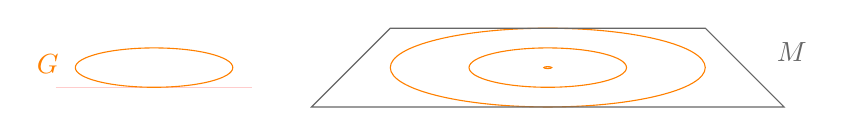
\begin{tikzpicture}
		\draw[red!20] (-6.25,.25) -- (-3.75,.25);
		\draw[orange] (-5,.5) ellipse (1 and .25);
		\node[orange] at (-6.35,.55) {$G$};

		\draw[orange] (0,.5) ellipse (.05 and .0125);
		\draw[orange] (0,.5) ellipse (1 and .25);
		\draw[orange] (0,.5) ellipse (2 and .5);
		\draw[black!60] (-3,0) -- (3,0) -- (2,1) -- (-2,1) -- cycle;
		\node[black!60] at (3.1,.7) {$M$};
	\end{tikzpicture}
	
	\vspace{5pt}
	\hspace{.75cm}we could describe the induced map ${\color{orange}\xi\mapsto\underline\xi}$ \ldots

	\vspace{5pt}
	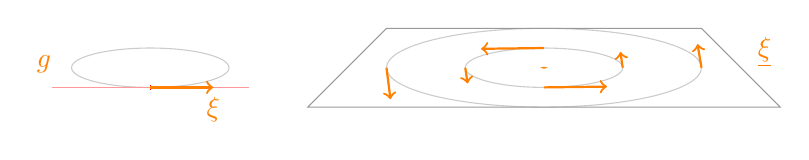
\begin{tikzpicture}
		\draw[black!20] (-5,.5) ellipse (1 and .25);
		\draw[red!40] (-6.25,.25) -- (-3.75,.25);
		\draw[red] (-5,.22) -- (-5,.28);
		\node[orange] at (-6.35,.55) {$\mathfrak{g}$};
		\draw[thick,orange,->] (-5,.25) -- (-4.2,.25) node[anchor=north] {$\xi$};

		\draw[black!20] (0,.5) ellipse (1 and .25);
		\draw[black!20] (0,.5) ellipse (2 and .5);
		\draw[black!40] (-3,0) -- (3,0) -- (2,1) -- (-2,1) -- cycle;

		\draw[orange,fill=red] (0,.5) ellipse (.02 and .02/4);

		\draw[thick,orange,->] (0,.25) -- (.8,.25+.01);
		\draw[thick,orange,->] (0,.75) -- (-.8,.75-.01);

		\draw[thick,orange,->] (1,.5) -- (.97,.7);
		\draw[thick,orange,->] (-1,.5) -- (-.97,.3);

		\draw[thick,orange,->] (2,.5) -- (2-.05,.8);
		\draw[thick,orange,->] (-2,.5) -- (-2+.05,.1);

		\node[orange] at (2.8,.7) {$\underline\xi$};
	\end{tikzpicture}

	\hspace{1.5cm} or an assignment of Hamiltonian functions ${\color{blue}\xi\mapsto f_{\underline\xi}}$.

	\vspace{5pt}
	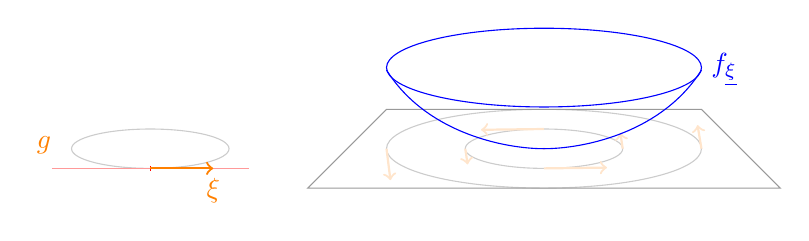
\begin{tikzpicture}
		\draw[black!20] (-5,.5) ellipse (1 and .25);
		\draw[red!40] (-6.25,.25) -- (-3.75,.25);
		\draw[red] (-5,.22) -- (-5,.28);
		\node[orange] at (-6.35,.55) {$\mathfrak{g}$};
		\draw[thick,orange,->] (-5,.25) -- (-4.2,.25) node[anchor=north] {$\xi$};

		\draw[black!20] (0,.5) ellipse (1 and .25);
		\draw[black!20] (0,.5) ellipse (2 and .5);
		\draw[black!40] (-3,0) -- (3,0) -- (2,1) -- (-2,1) -- cycle;

		\draw[red!20] (0,.5) ellipse (.02 and .02/4);

		\draw[thick,orange!20,->] (0,.25) -- (.8,.25+.01);
		\draw[thick,orange!20,->] (0,.75) -- (-.8,.75-.01);

		\draw[thick,orange!20,->] (1,.5) -- (.97,.7);
		\draw[thick,orange!20,->] (-1,.5) -- (-.97,.3);

		\draw[thick,orange!20,->] (2,.5) -- (2-.05,.8);
		\draw[thick,orange!20,->] (-2,.5) -- (-2+.05,.1);

		\draw[blue] (0,1.53) ellipse (2 and .5);

		\draw[blue] (0,.5) .. controls (.5,.5) and (1.5,.7) .. (2,1.5) node[anchor=west] {$f_{\underline\xi}$};
		\draw[blue] (0,.5) .. controls (-.5,.5) and (-1.5,.7) .. (-2,1.5);
	\end{tikzpicture}

	\vspace{-4pt}
	When this is possible\footnote{\color{black!50}\tiny{*and $\xi\mapsto f_{\underline\xi}$ is a homomorphism of Lie algebras}}, the action is called \textbf{Hamiltonian}.
	
\end{frame}
%------------------------------------------------------------------------------------------------

%------------------------------------------------------------------------------------------------
\begin{frame}\frametitle{Symplectic Reduction --- Idea}
	\[
		\omega = \underbrace{\;\d x_1\wedge\d y_1\;}_{\text{to be removed}}\hspace{3pt}+\hspace{5pt}  \d x_2\wedge\d y_2 + \cdots +\d x_n\wedge\d y_n
	\]

	\begin{center}
	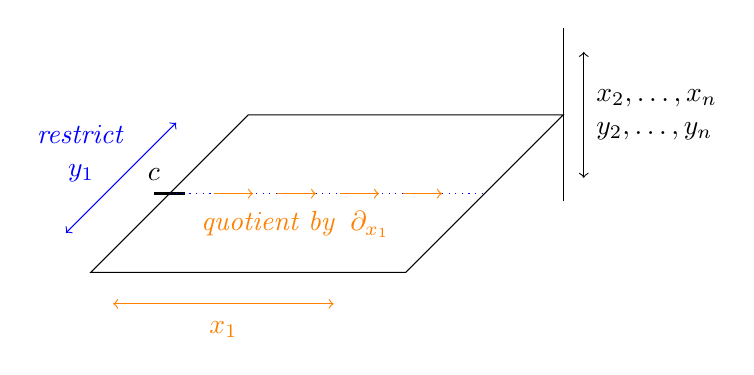
\begin{tikzpicture}[scale=2]	
		\draw (0,0) -- (2,0) -- (3,1) -- (1,1) -- cycle;
		\draw[<->,orange,xshift=-4.5pt] (.3,-.2) -- node[below=3pt,align=center] {$x_1$} (1.7,-.2);
		\draw[<->,blue,xshift=-4.5pt] (0,.25) -- node[above left=-5pt,align=center] {\emph{restrict}\\$y_1$} +(.7,.7);
		
		\draw[black,thick] (.5,.5) +(-.1,0) node[above=1pt] {$c$} -- +(.1,0);
		\draw[blue,dotted] (.5,.5) -- node[pos=.4,below=3pt,orange] {\emph{quotient by} \,$\partial_{x_1}$} (2.5,.5);

		\draw[orange,->] (.78,.5) -- +(.25,0);
		\draw[orange,->] (1.18,.5) -- +(.25,0);
		\draw[orange,->] (1.58,.5) -- +(.25,0);
		\draw[orange,->] (1.98,.5) -- +(.25,0);

		\draw (3,.45) -- (3,1.55);
		\draw[<->] (3.13,.6) -- node[right=1pt,align=left] {$x_2, \ldots ,x_n$\\$y_2, \ldots ,y_n$} (3.13,1.4);
	\end{tikzpicture}
	\end{center}
	
	\begin{center}
		\emph{{\color{blue}Restrict} and {\color{orange}quotient} conjugate degrees of freedom.}
	\end{center}
\end{frame}
%------------------------------------------------------------------------------------------------

%------------------------------------------------------------------------------------------------
\begin{frame}\frametitle{Symplectic Reduction --- Proof}
	\begin{center}
	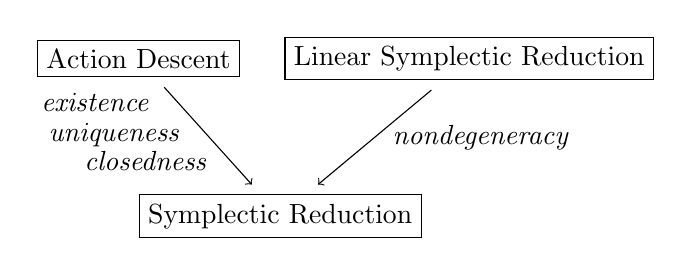
\begin{tikzpicture}
		\node (A) at (-2,2) {\fbox{Action Descent}};
		\node (B) at (2.2,2) {\fbox{Linear Symplectic Reduction}};
		\node (C) at (-.2,0) {\fbox{Symplectic Reduction}};

		\draw[->] (A)--(C);
		\draw[->] (B)-- node[right=3pt] {\emph{nondegeneracy}} (C);

		\node at (-2.54,1.44) {\emph{existence}};
		\node at (-2.3,1.03) {\emph{uniqueness}};
		\node at (-1.9,.7) {\emph{closedness}};
	\end{tikzpicture}
	\end{center}

	\vspace{-.3cm}
	\begin{enumerate}
		\item Apply the \emph{Action Descent Lemma} to $G_\lambda\curvearrowright\mu^{-1}(\lambda)$ and $i^*\omega$.
			\begin{center}
			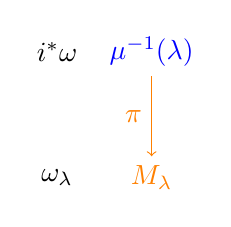
\begin{tikzpicture}[scale=2]
				\node[blue] (A) at (0,0) {$\mu^{-1}(\lambda)$};
				\node (A2) at (-.6,0) {$i^*\omega$};
				\node[orange] (C) at (0,-.8) {$M_\lambda$};
				\node (C2) at (-.6,-.8) {$\omega_\lambda$};

				\path[->,orange] (A) edge node[left] {$\pi$} (C);
			\end{tikzpicture}
			\end{center}

		\item Use \emph{Linear Symplectic Reduction} to conclude that $\omega_\lambda$ is nondegenerate.
	\end{enumerate}
\end{frame}
%------------------------------------------------------------------------------------------------

%------------------------------------------------------------------------------------------------
\begin{frame}\frametitle{The Action Descent Lemma}
	\begin{lemblock}
	If
	\begin{itemize}
		\item $G\curvearrowright M$ free and proper,
		\item $\alpha\in\Omega^*(M)$ \emph{invariant} and \emph{horizontal} ($\iota_{\underline\g}\hspace{1pt}\alpha=0$),
	\end{itemize}

	\vspace{-.3cm}
	\begin{center}
	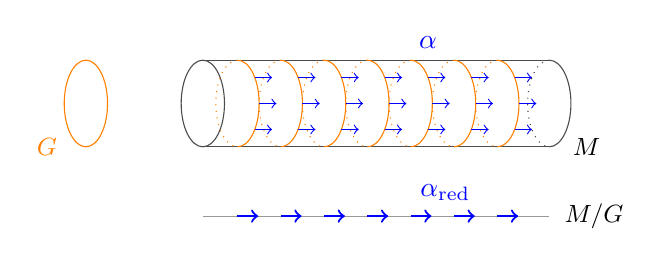
\begin{tikzpicture}[scale=1.1]
		\draw[yshift=-.8cm,black!40] (0,0) -- (4,0) node[black,right=2pt] {\small $M/G$};

		\begin{scope}[xshift=-1.35cm]
		\draw[orange] (0,.5) ellipse (.25 and .5);
		\end{scope}

		\node[orange] at (-1.8,0) {\small $G$};

		\node[orange] at (-.7,.5) {$\curvearrowright$};

		\draw[black!70] (0,.5) ellipse (.25 and .5);
		\draw[black!70] (4,0) arc (-90:90:.25 and .5);
		\draw[dotted,black!70] (4,1) arc (90:270:.25 and .5);
		\draw[black!70] (0,0) -- (4,0) node[black,right=5pt] {\small $M$};
		\draw[black!70] (0,1) -- (4,1);

		\foreach \x in {-1,-.5,...,2}
		{
			\begin{scope}[xshift=\x cm]
				\draw[orange,xshift=1.4cm] (0,0) arc (-90:90:.25 and .5);
				\draw[orange,dotted,xshift=1.4cm] (0,1) arc (90:270:.25 and .5);

				\draw[blue,->,shift={(1.7,.2)}] (-.1,0) -- (.1,0);
				\draw[blue,->,shift={(1.7,.8)}] (-.1,0) -- (.1,0);
				\draw[blue,->,shift={(1.75,.5)}] (-.1,0) -- (.1,0);
			\end{scope}

			\begin{scope}[xshift=\x cm]
				\draw[blue,->,thick,shift={(1.5,-.8)}] (-.1,0) -- (.14,0);
			\end{scope}
		}

		\node[blue] at (2.6,1.2) {$\alpha$};
		\node[blue] at (2.8,-.53) {$\alpha_{\mathrm{red}}$};
	\end{tikzpicture}
	\end{center}
	\vspace{-.4cm}
	then
	\begin{itemize}
		\item $\exists ! \,\alpha_{\mathrm{red}}\in\Omega^*(M/G)$ such that $\alpha=\pi^*\alpha_{\mathrm{red}}$,
		\item $\d\alpha=0 \implies \d\alpha_{\mathrm{red}}=0$.
	\end{itemize}
	\end{lemblock}	

\end{frame}
%------------------------------------------------------------------------------------------------



%------------------------------------------------------------------------------------------------
\begin{frame}\frametitle{The Space of Moment Maps}
	\vspace{-.2cm}
	\begin{itemize}
		\item $(M,\omega,G,\mu)$ Hamiltonian $G$-space
		\item $\phi\in\Omega^{k-1}(M,\g^*)$
	\end{itemize}

	\vspace{.3cm}
	\emph{Question:} When is $\mu+\phi$ a moment map?
	\vspace{.3cm}

	\begin{itemize}
		\item ${\color{green}\d\phi=0}$, since
			\[
				\d(\mu+\phi)_\xi = \iota_\xi\omega \iff \d\phi_\xi=0.
			\]
		\item ${\color{green}\L_\xi\phi_\zeta=\phi_{[\xi,\zeta]}}$, as
			\[
				\L_\xi (\mu+\phi) = (\mu+\phi)_{[\xi,\zeta]} \iff \L_\xi\phi = \phi_{[\xi,\zeta]}.
			\]
	\end{itemize}
	
	\vspace{.2cm}
	i.e.\ $\phi$ is a moment map for the trivial action $G\curvearrowright M$.

	\vspace{.2cm}
	{\tiny The space of moment maps is an affine space modeled on $\{\phi\in\Omega^{k-1}(M,\g^*)\,|\,\d\phi=0,\;G_\phi=G\}$.}
\end{frame}

\begin{frame}\frametitle{The Leibniz Condition and the Induced Action on Forms}
	\vspace{-.2cm}
	\begin{itemize}
		\item $\phi\in\Omega^*(M,\g^*)$
		\item $\xi\in\g$
	\end{itemize}

	\vspace{-.4cm}
	\begin{align*}
		{\color{black!40}\forall\zeta\in\g:\hspace{.3cm}}\L_\xi\phi_\zeta=\phi_{[\xi,\zeta]}	&&{\color{black!40}\iff\forall\zeta\in\g:}
					&&0	&=	\L_\xi\phi_\zeta - \phi_{[\xi,\zeta]}			\\
					&&						&&	&=	\L_\xi\phi_\zeta + \langle\mathrm{ad}_\xi^*\phi,\zeta\rangle\\
					&&						&&	&=	\langle\L_\xi\phi + \mathrm{ad}_\xi^*\phi,\zeta\rangle	\\
					&&						&&	&	\\[-8pt]
					&&	{\color{black!40}\iff}\hspace{.3cm}	&&0	&=	(\L_\xi + \mathrm{ad}_\xi^*)\hspace{2pt}\phi					\\
					&&						&&	&	\\[-8pt]
					&&	{\color{black!40}\iff}\hspace{.3cm}	&&\xi	&\in	\g_\phi
	\end{align*}
	in terms of the induced action $G\curvearrowright\Omega^*(M,\g^*)$. Thus,
	\[
		{\color{black!40}\forall\xi,\zeta\in\g:\hspace{.3cm}}\L_\xi\phi_\zeta=\phi_{[\xi,\zeta]}	\hspace{.3cm}{\color{black!40}\iff}\hspace{.3cm}	G\cdot\phi = \phi
	\]
\end{frame}

\begin{frame}\frametitle{Level Sets of the Moment Map}
	Rather than:
	\begin{itemize}
		\item {\color{green}family of moment maps} $\{\mu-\phi\,|\,\d\phi=0,\;G_\phi=G\}$
		\item reduction at $\mu-\phi=0$
	\end{itemize}


	\vspace{.5cm}
	We instead consider:
	\begin{itemize}
		\item fixed moment map $\mu$
		\item {\color{green}family of levels} $\{\phi\,|\,\d\phi=0,\;\text{\sout{$G_\phi=G$}}\}$
		\item reduction at $\mu=\phi$
	\end{itemize}

	\vspace{.5cm}
	%The \emph{level set} associated to $\phi$ is
	\emph{$\phi$-level set:}
	\[
		\mu^{-1}(\phi) := \{\mu=\phi\}
	\]
\end{frame}


%%%%% MULTISYMPLECTIC REDUCTION

\begin{frame}\frametitle{Multisymplectic Reduction --- Proof Idea}
	\begin{center}
	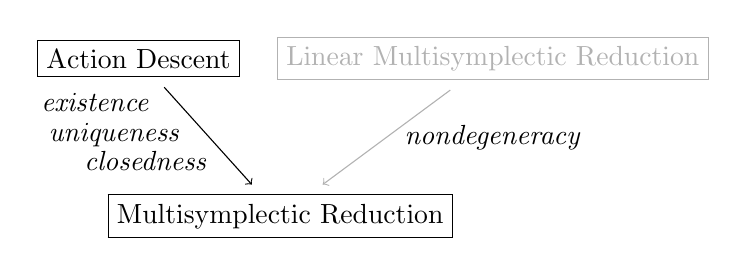
\begin{tikzpicture}
		\node (A) at (-2,2) {\fbox{Action Descent}};
		\node[black!30] (B) at (2.5,2) {\fbox{\sout{Linear Multisymplectic Reduction}}};
		\node (C) at (-.2,0) {\fbox{Multisymplectic Reduction}};

		\draw[->] (A)--(C);
		\draw[->,black!30] (B)-- node[right=3pt,black] {\sout{\emph{nondegeneracy}}} (C);

		\node at (-2.54,1.44) {\emph{existence}};
		\node at (-2.3,1.03) {\emph{uniqueness}};
		\node at (-1.9,.7) {\emph{closedness}};
	\end{tikzpicture}
	\end{center}

	\vspace{-.3cm}
	\begin{enumerate}
		\item Apply the \emph{Action Descent Lemma} to $G_\phi\curvearrowright\mu^{-1}(\phi)$ and $i^*\omega$.
			\begin{center}
			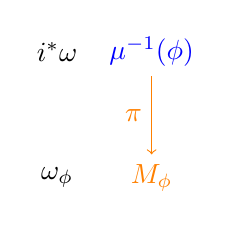
\begin{tikzpicture}[scale=2]
				\node[blue] (A) at (0,0) {$\mu^{-1}(\phi)$};
				\node (A2) at (-.6,0) {$i^*\omega$};
				\node[orange] (C) at (0,-.8) {$M_\phi$};
				\node (C2) at (-.6,-.8) {$\omega_\phi$};

				\path[->,orange] (A) edge node[left] {$\pi$} (C);
			\end{tikzpicture}
			\end{center}

		\item {\color{black!30}\sout{Use \emph{Linear Multisymplectic Reduction} to conclude that $\omega_\phi$ is nondegenerate.}}
	\end{enumerate}
\end{frame}

\begin{frame}\frametitle{Multisymplectic Reduction --- Proof Outline}
	Two steps:
	\begin{enumerate}
		\item ${\color{orange}G_\phi\curvearrowright M}$ preserves ${\color{blue}\mu^{-1}(\phi)}$,
		\item $i^*\omega$ is invariant and horizontal.
	\end{enumerate}
\end{frame}

\begin{frame}\frametitle{Multisymplectic Reduction --- Proof (Step 1)}
	\begin{enumerate}
		\item {\color{orange}$G_\phi\curvearrowright M$} preserves {\color{blue}$\mu^{-1}(\phi)$}.
	\end{enumerate}

	\vspace{.4cm}
	\begin{itemize}
		\item $\mu^{-1}(\phi) = \{\mu-\phi=0\}$

		\vspace{.4cm}
		\item {\color{black}$\forall\,\xi,\zeta\in\g_\phi$,}
			\vspace{-.2cm}
			\begin{align*}
				\L_\xi\hspace{1pt} (\mu-\phi)_\zeta
					&=	(\mu-\phi)_{[\xi,\zeta]},	&&\hspace{-.2cm}\text{by the Leibniz condition,}	\\
					&=	0				&&\hspace{-.2cm}\text{on $\mu^{-1}(\phi)$.}
			\end{align*}
	\end{itemize}
\end{frame}

\begin{frame}\frametitle{Multisymplectic Reduction --- Proof (Step 2)}
	\begin{enumerate}\setcounter{enumi}{1}
		\item $i^*\omega$ is invariant and horizontal.
	\end{enumerate}

	\vspace{.2cm}

	\begin{itemize}
		\item \textbf{invariant:} Hamiltonian actions are multisymplectic.\\[3pt]
		\item \textbf{horizontal:} For $\xi\in\g_\phi$,
		\begin{align*}
			\iota_\xi i^*\omega
				&=	i^* {\color{red}\iota_\xi\omega},	&&\hspace{-1cm}\text{since ${\color{orange}G_\phi}$ preserves ${\color{blue}\mu^{-1}(\phi)}$,}		\\
				&=	i^* {\color{red}\d\mu_\xi},	&&\hspace{-1cm}\text{by the Hamiltonian condition,}	\\
				&=	i^* \d\phi_\xi,			&&\hspace{-1cm}\text{since ${\color{blue}\mu=\phi}$ on ${\color{blue}\mu^{-1}(\phi)}$,}		\\
				&=	0,					&&\hspace{-1cm}\text{as ${\color{blue}\phi}$ is closed.}
		\end{align*}
	\end{itemize}
	\hspace*{\fill}$\qed$
\end{frame}


%%%%%  REDUCTION OF CLOSED FORMS

\begin{frame}\frametitle{Extension: Reduction of Closed Forms}
	\begin{enumerate}
		\item The proof makes no use of the nondegeneracy or homogeneity of $\omega\in\Omega^{k+1}(M)$.
		\item Extends naturally to a reduction scheme for closed forms.
	\end{enumerate}

	\vspace{-.3cm}
	\begin{align*}
		\omega	&\in\Omega^*(M) \text{ closed}		\\
		\phi	&\in\Omega^*(M,\g^*) \text{ closed}
	\end{align*}

	\vspace{-.4cm}
	\begin{align*}
				&\hspace{-.8cm}\underline{\mu\in\Omega^*(M,\g^*)}	\\
		\d\mu_\xi	&=	\iota_\xi\omega					\\
		\L_\xi\mu_\zeta	&=	\mu_{[\xi,\zeta]}
	\end{align*}
\end{frame}
%------------------------------------------------------------------------------------------------


%------------------------------------------------------------------------------------------------
\end{document}

	




%- HandOut Flag -----------------------------------------------------------------------------------------
\newif\ifHandout
%	\Handouttrue  %uncomment for the printable version

%- D0cum3nt ----------------------------------------------------------------------------------------------
\documentclass[beamer,handout,10pt]{standalone}   
\ifHandout
	\setbeameroption{show notes} %print notes   
\fi

	
%- Packages ----------------------------------------------------------------------------------------------
\usepackage{custom-style}

%--Beamer Style-----------------------------------------------------------------------------------------------
\usetheme{toninus}








%---------------------------------------------------------------------------------------------------------------------------------------------------
%- D0cum3nt ----------------------------------------------------------------------------------------------------------------------------------
\begin{document}
%------------------------------------------------------------------------------------------------


\subsection{References}

%------------------------------------------------------------------------------------------------
% https://en.wikibooks.org/wiki/LaTeX/Bibliographies_with_biblatex_and_biber
\begin{frame}[t,allowframebreaks]{Extended Bibliography}
	%\nocite{*}
	\bibliographystyle{alpha}
	\bibliography{bibfile}
\end{frame}
%------------------------------------------------------------------------------------------------





%------------------------------------------------------------------------------------------------
\begin{frame}[t,allowframebreaks]{Pictures - Credits}
	\begin{itemize}
		\item MW reduction as "restriction to level sets", C. Lessig,
			\href{https://arxiv.org/abs/1206.3302}{arXiv:1206.3302}
	\end{itemize}
\end{frame}
%------------------------------------------------------------------------------------------------



%------------------------------------------------------------------------------------------------
\end{document}
%------------------------------------------------------------------------------------------------










%------------------------------------------------------------------------------------------------
\end{document}

